% -*- TeX -*- -*- Soft -*-
% -*- TeX -*- -*- Soft -*-
% -*- TeX -*- -*- Soft -*-
% -*- TeX -*- -*- Soft -*-
\input{galop08.pre}
\usepackage{graphicx}
\usepackage{url}
\def\toolname{HOG}


\title{A tool illustrating the Correspondence Theorem
\\ GALOP 2008}

\author{William~Blum~~~~~~~~~~~C.-H.~Luke~Ong\\
Oxford University Computing Laboratory\\
Wolfson Building, Parks Road, Oxford OX1 3QD, ENGLAND\\
\{william.blum,luke.ong\}@comlab.ox.ac.uk }



\begin{document}
\maketitle \thispagestyle{empty}

\begin{abstract}
Todo...
\end{abstract}

\tableofcontents

\section{Luke's description of the paper:}

 We have developed a number of what we call Path-Traversal
Correspondence Theorems. One way to think of the work is as a kind of representation theory of the game semantics of higher-type programs (such as recursion schemes, PCF and Idealized Algol) that is very concrete, involving combinatorics over (possibly) infinite structures defined by the abstract syntax trees of the programs being modelled. The idea is that we represent a play in the strategy-denotation of a term as the underlying "hereditarily uncovered" interaction sequence, called traversal. Another way to put it is that traversals are built up by performing parallel-composition but WITHOUT the hiding. This is what William Greenland has called (in his thesis) "revealed semantics" (or "interaction semantics"). A consequence of the representation is that we show how the "innocent game" given by a term can be played out very concretely over what is in essence the abstract syntax tree of the term itself.

This "representation theory" was first developed to prove the result in my LICS06 paper (i.e. trees generated by higher-order recursion schemes have decidable MSO theories). The theory has at least two other applications. First as a justification of the game characterization of the Higher-Order Matching Problem (but NOT the algorithm) developed by Colin Stirling, and secondly as a key lemma underpinning the result that
 the following are equivalent (i.e. equi-expressive:
i. order-n recursion schemes (= order-n PCF terms generated from uninterpreted order-1 symbols) ii. order-n collapsible pushdown automata CPDA. iii. order-n "pure" innocent strategies

What we are thinking of submitting is a short paper describing a tool developed by William Blum that illustrates the representation theory. The tool has many capabilities. For example, it can perform the inter-translation between CPDA and recursion schemes; it can demonstrate the path-traversal correspondence in the form of a 2-player game (and lets users play it out over the abstract syntax tree of the term); and it is a very impressive tool for drawing justified sequences!

What we intend to talk about in the paper is first an overview of the correspondence theorems, illustrate their many applications, and then showcase the tool.

\section{Computation tree, Traversals and the Correspondence Theorem}

In \cite{OngLics2006}, one of us introduced the notion of computation tree and traversals over a computation tree for the purpose of studying trees generated by higher-order recursion scheme. Here we extend these concepts to the pure (\ie without constants) simply-typed lambda calculus. Our setting allows the presence of free variable of any order. Moreover the term studied is not necessarily of ground type. (This contrasts with \cite{OngLics2006}'s setting where the term is of ground type and contains only \emph{uninterpreted constant}\footnote{A constant $f$ is  \emph{uninterpreted} if the small-step semantics of the language
  does not contain any rule of the form $f \dots \rightarrow e$. $f$
  can be regarded as a data constructor.} of order 1 at most and no
free variables.) Note that our setting automatically accounts for the presence of uninterpreted constants since they can be regarded as free variables. We will then state the \emph{Correspondence Theorem} (Theorem \ref{thm:correspondence}).

In the following we fix a simply-typed term $\Gamma \vdash M :T$.

\subsection{Computation tree}
 In \cite{OngLics2006} the computation tree of a grammar is
defined as the unravelling of a finite graph representing the long transform of a grammar. Similarly we define the computation tree of a $\lambda$-term as an abstract syntax tree of its $\eta$-long normal form.  We write $l\langle t_1, \ldots, t_n \rangle$ with $n \geq 0$ to denote the tree with a root labelled $l$ with $n$ children subtrees $t_1$, \ldots, $t_n$.

\begin{definition}\rm
\label{dfn:comptree}
  The \defname{computation tree} $\tau(M)$ of a simply-typed term
  $\Gamma \vdash M:T$ with variable names in a countable set
  $\mathcal{V}$ is a tree with labels in $ \{ @ \} \union \mathcal{V}
  \union \{ \lambda x_1 \ldots x_n \ | \ x_1 ,\ldots, x_n \in
  \mathcal{V}, n\in\nat \}$ defined from its $\eta$-long form as follows.
  Let $\overline{x}$ denote some list of variables $x_1 \ldots x_n$ for some $n\geq 0$.
\begin{eqnarray*}
  \mbox{For $m\geq 0$, $z \in \mathcal{V}$: } \tau(\lambda \overline{x} . z s_1 \ldots s_m ) &=& \lambda \overline{x} \langle z \langle\tau(s_1),\ldots,\tau(s_m)\rangle\rangle \\
  \mbox{For $m \geq 1$: } \tau(\lambda \overline{x} . (\lambda y.t) s_1 \ldots s_m) &=& \lambda \overline{x} \langle @ \langle \tau(\lambda y.t),\tau(s_1),\ldots,\tau(s_m) \rangle \rangle \ .
\end{eqnarray*}
\end{definition}

Even-level nodes are $\lambda$-nodes (the root is on level 0). A single $\lambda$-node can represent several consecutive variable abstractions or it can just be a \emph{dummy lambda} if the corresponding subterm is of ground type.  Odd-level nodes are variable or application nodes.

We say that a variable node $n$ labelled $x$ is \defname{bound} by a node $m$, and $m$ is called the \defname{binder} of $n$, if $m$ is the closest node in the path from $n$ to the root such that $m$ is labelled $\lambda \overline{\xi}$ with $x\in \overline{\xi}$.


We write $\theroot$ to denote the root of the computation tree $\tau(M)$. The set of nodes of the computation tree is denoted by $N$. The sets $N_@$, $N_\lambda$ and $N_{\sf var}$ are the subset of $N$ consisting of the @-nodes, $\lambda$-nodes and variable nodes respectively.


\subsection{Justified sequences of nodes}

We define the \defname{enabling relation} on the set of nodes of the computation tree as follows: $m$ enables $n$, written $m \vdash n$, if and only if $n$ is bound by $m$ (and we sometimes write $m \vdash_i n$ to precise that $n$ is the $i^{\sf th}$ variable bound by $m$); or $m$ is the root $\theroot$ and $n$ is a free variable; or $n$ is a $\lambda$-node and $m$ is its parent node.


We say that a node $n_0$ of the computation tree is
\defname{hereditarily enabled} by $n_p \in N$ if there are nodes
$n_1,\ldots, n_{p-1} \in N$ such that $n_{i+1}$ enables $n_{i}$ for all $i\in 0..p-1$.

For any set of nodes $S, H \subseteq N$ we write $S^{H\vdash}$ for $S \inter \vdash^*(H) = \{ n \in S \ | \exists n_0 \in H \mbox{ s.t. }n_0  \vdash^* n \}$ -- the subset of $S$ constituted of nodes hereditarily enabled by some node in $H$. We will abbreviate $S^{\{n_0\}\vdash}$ into $S^{n_0\vdash}$.

We call \defname{input-variables nodes} the elements of $V_{\sf var}^{\theroot\vdash}$ \ie variables that are hereditarily enabled by the root of $\tau(M)$. Thus we have $V_{\sf var}^{\theroot\vdash} = V \setminus ( V_{\sf var}^{N_@\vdash} \union V_{\sf var}^{N_\Sigma\vdash})$.

A \defname{justified sequence of nodes} is a sequence of nodes with pointers such that each occurrence of a variable or $\lambda$-node $n$ different from the root has a pointer to some preceding occurrence $m$ verifying $m \vdash n$. In particular, occurrences of @-nodes do not have pointer. We represent the pointer in the sequence as follows \Pstr[0.4cm]{ (m){m} \ldots (n-m,45:i) n }.
 where the label indicates that either $n$ is labelled with the $i$th variable
abstracted by the $\lambda$-node $m$ or that $n$ is the $i^{\sf th}$ child of $m$.  Children nodes are numbered from $1$ onward except for @-nodes where it starts from $0$. Abstracted variables are numbered from $1$ onward. The $i^{\sf th}$ child of $n$ is denoted by $n.i$.

We say that a node $n_0$ of a justified sequence is
\defname{hereditarily justified} by $n_p$ if there are occurrences $n_1,
\ldots, n_{p-1}$ in the sequence such that $n_i$ points to $n_{i+1}$ for all $i\in 0..p-1$. Let $n$ be an occurrence in a justified sequence $s$. We write $s \filter r$ to denote the subsequence of $s$ consisting of the occurrences hereditarily justified by $n$.


The notion of \defname{P-view} $\pview{t}$ of a justified sequence of nodes $t$ is defined the same way as the P-view of a justified sequences of moves in Game Semantics:\footnote{ The equalities in the
  definition determine pointers implicitly. For instance in the second
  clause, if in the left-hand side, $n$ points to some node in $s$
  that is also present in $\pview{s}$ then in the right-hand side, $n$
  points to that occurrence of the node in $\pview{s}$.}
$$\begin{array}{rclrcl}
\pview{\epsilon} &=&  \epsilon & \pview{\Pstr[0.5cm]{ s \cdot (m) m \cdot \ldots \cdot (lmd-m,40){\lambda\overline{\xi}} }}
 &=& \Pstr{
\pview{s} \cdot (m2) m \cdot (lm2-m2,50) {\lambda \overline{\xi}} } \\
\mbox{for $n \notin N_\lambda$, } \pview{s \cdot n }  &=&  \pview{s} \cdot n \qquad & \pview{s \cdot \theroot }  &=&  \theroot
\end{array}$$

The O-view of $s$, written $\oview{s}$, is defined dually. We will borrow the game semantic terminology: A justified sequences of nodes satisfies \defname{alternation} if for any two consecutive nodes one is a $\lambda$-node and the other is not, and \defname{P-visibility} if every variable node points to a node occurring in the P-view a that point.

\subsection{Adding value-leaves to the computation tree}

We now add another ingredient to the computation tree that was not originally used in \cite{OngLics2006}.  We write $\mathcal{D}$ to denote the set of values of the base type $o$.  We add
\defname{value-leaves} to $\tau(M)$ as follows: For each value $v
\in \mathcal{D}$ and for each node $n \in N$ we attach the child leaf $v_n$ to $n$.  We write $V$ for the set of vertices of the resulting tree (\ie inner nodes and leaf nodes). For $\$$ ranging in $\{@, \lambda, var \}$, we write $V_\$$ to denote the set of inner nodes from $N_\$$ plus the leaf-nodes whose parent is in $N_\$$ \ie $V_\$ = N_\$ \union \{ v_n \ | \ n \in N_\$, v \in \mathcal{D} \}$.


Everything that we have defined can be lifted to this new version of computation tree. The enabling relation $\vdash$ is extended so that every leaf is enabled by its parent node. A link going from a value-leaf $v_n$ to a node $n$ is labelled by $v$: \Pstr[0.4cm]{ (n) n \ldots (vn-n,35:v){v_n} }. For the definition of P-view and visibility, value-leaves are treated as $\lambda$-nodes if they are at an odd level in the computation tree, and as variable nodes if they are at an even level.

We say that an occurrence of an inner node $n \in N$ is
\defname{answered} by an occurrence $v_n$ if $v_n$ in
the sequence that points to $n$, otherwise we say that $n$ is
\defname{unanswered}. The last unanswered node is called the
\defname{pending node}.  A justified sequence of nodes is
\defname{well-bracketed} if each value-leaf occurring in it is justified by the pending node at that point.  If $t$ is a traversal then we write
$?(t)$ to denote the subsequence of $t$ consisting only of unanswered nodes.

\subsection{Traversals of the computation tree}
\label{subsec:traversal}

A \emph{traversal} is a justified sequence of nodes of the computation tree where each node indicates a step that is taken during the evaluation of the term.

\input{../thesis/traversal_rules_def}

\parpic[r]{
 $\pssetcomptree\tree[levelsep=3ex,treesep=0.5cm]{\lambda} {
    \tree{@}{
        \pstree[linestyle=dotted]{\TR{\lambda y}\arclabel{0} }{
            \tree{y}{
                \tree{\lambda \overline{\eta_1}}{\vdots}%\arclabel{1}
                \tree{\lambda \overline{\eta_i}}{\vdots}%\arclabel{i}
                \tree{\lambda \overline{\eta_n}}{\vdots}%\arclabel{n}
            }
        }
        \pstree[linestyle=dotted]{\TR{\lambda \overline{x}}
            \arclabel{1}}{ \tree{x_i}{\TR{} \TR{}}}
}}$ } A traversal always starts by visiting the root. Then it mainly follows the structure of the tree. The (Var) rule permits to jump across the computation tree. The idea is that after visiting a variable node $x$, a jump is allowed to the node corresponding to the subterm that would be substituted for $x$ if all the $\beta$-redexes occurring in the term were reduced. The sequence \Pstr[0.8cm]{\lambda \cdot (app) @  \cdot (ly) {\lambda y}  \ldots (y-ly,35:1) y  \cdot (lx-app,38:1) {\lambda \overline{x}} \ldots (x-lx,30:i) {x_i} \cdot (leta-y,40:i) {\lambda \overline{\eta_i} } \ldots}
 is an example of traversal of the computation tree shown on the right.

\begin{proposition}[counterpart of proposition 6 from \cite{OngHoMchecking2006}]
\label{prop:pviewtrav_is_path} Let $t$ be a traversal. Then:
\begin{enumerate}[(i)]
\item $t$ is a well-defined and well-bracketed justified sequence;
\item $t$ is a well-defined justified sequence verifying alternation, P-visibility and O-visibility;
\item If $t$'s last node is not a value-leaf, then $\pview{t}$ is the path in the computation tree going from the root to $t$'s last node.
\end{enumerate}
\end{proposition}

The \defname{reduction} of a traversal $t$ is the subsequence of $t$ obtained by keeping only occurrences of nodes that are hereditarily enabled by the root $\theroot$. This has the effect of eliminating the ``internal nodes'' of the computation. If $t$ is a non-empty traversal then the root $\theroot$ occurs exactly once in $t$ and the reduction of $t$ is equal to $t \filter r$. We write $\travset(M)^{\filter \theroot}$ for the set or reduction of traversals of $M$.

Application nodes are used to connect the operator and the operand of an application in the computation tree but since they do not play any role in the computation of the term, we can remove them from the traversals.  We write $t-@$ for the sequence of nodes-with-pointers obtained by removing from $t$ all @-nodes and value-leaves of @-nodes, any link pointing to an @-node being replaced by a link pointing to the immediate predecessor of @ in $t$. We write $\travset(M)^{-@}$ for the set $\{ t - @ \ | \  t \in \travset(M) \}$.
\begin{remark}
If $M$ is $\beta$-normal then $\tau$ does not contain any @-node therefore all nodes are hereditarily justified by $r$ and we have $\travset(M)^{-@} = \travset(M) = \travset(M)^{\filter \theroot }$.
\end{remark}

\subsection{Revealed Game Semantics}

In game semantics, strategy composition is achieved by performing a CSP-like ``composition + hiding''. If the internal moves are not hidden then we obtain an alternative semantics called \emph{revealed semantics} in \cite{willgreenlandthesis} and \emph{interaction} semantics in \cite{DBLP:conf/sas/DimovskiGL05}. Here we will refer to this semantics as the \defname{fully revealed game semantics}. The fully revealed game denotation of a term $\Gamma \vdash M :T$, written $\revsem{\Gamma \vdash M : T}$, is obtained by uncovering\footnote{An algorithm that uniquely recovers hidden moves is given in Part II of
  \cite{hylandong_pcf}.} all the internal moves from $\sem{\Gamma \vdash
  M : T}$ generated during strategy composition.
We introduce a variation of the fully-revealed game denotation called the \defname{syntactically-revealed game denotation}, written $\syntrevsem{\Gamma \vdash
  M : T}$. In this denotation, as opposed to the fully-revealed denotation,
only \emph{certain} internal moves from $\sem{\Gamma \vdash
  M : T}$ are uncovered: The internal moves that are generated by the composition with the evaluation map
$ev$ at a @-node of the computation tree are all uncovered, but in the denotation of a subtem of the form $y N_1 \ldots N_p$ for some $p\geq1$, only certain internal moves are uncovered. The formal definition can be found in \cite{localbeta2008}.

\subsection{Computation trees and arenas}
We consider the well-bracketed game model of the simply-typed lambda calculus.  We choose to represent strategies using ``prefix-closed set of plays''. \footnote{In the literature, a strategy is usually defined as a set of plays closed by \emph{even}-length prefix. For the purpose of showing the Correspondence Theorem, however, the ``prefix-closed''-based definition is more adequate.} We fix a term $\Gamma \vdash M : T$ and write $\sem{\Gamma \vdash M : T}$ for its strategy denotation. The answer moves of a question $q$ are written $v_q$ where $v$ ranges in $\mathcal{D}$.

\begin{proposition}
There exists a function $\varphi_M$, constructible from $\tau(M)$, that maps nodes from $V\setminus (V_@ \union V_\Sigma)$ to moves of the interaction arena underlying the revealed strategy $\syntrevsem{\Gamma \vdash M : T}$ and such that $\varphi$ maps $\lambda$-nodes to O-questions, variable nodes to P-questions, value-leaves of $\lambda$-nodes to P-answers and value-leaves of variable nodes to O-answers.
\end{proposition}

\begin{example}
Take $\lambda x . (\lambda g . g x) (\lambda y . y)$ with $x,y:o$ and $g:(o,o)$. The diagram below represents the computation tree (middle), the arenas $\sem{(o,o), o}$ (left), $\sem{o , o}$ (right), $\sem{o\rightarrow o}$ (rightmost) and $\varphi = \psi \union \psi_{\lambda g.g x}^{\lambda g, q_{\lambda g}} \union \psi_{\lambda y.y}^{\lambda y, q_{\lambda y}}$ (dashed-lines).
$$\psset{levelsep=3.5ex}
\pstree{\TR[name=root]{\lambda x}} {
    \pstree{\TR[name=App]{@}}
    {
            \pstree{\TR[name=lg]{\lambda g}}
                { \pstree{\TR[name=lgg]{g}}{
                        \pstree{\TR[name=lgg1]{\lambda}}
                        { \TR[name=lgg1x]{x}  } } }
            \pstree{\TR[name=ly]{\lambda y}}
                    {\TR[name=lyy]{y}}
    }
} \rput(4.5cm,-1cm){
  \pstree{\TR[name=A1lx]{q_{\lambda x}}}
        { \TR[name=A1x]{q_x} }
} \rput(-6cm,-1.5cm){
    \pstree{\TR[name=A2lg]{q_{\lambda g}}}
    {
        \pstree{\TR[name=A2g]{q_g}}
        {  \TR[name=A2g1]{q_{g_1}}   }
    }}
\rput(2.5cm,-1.5cm){
    \pstree{\TR[name=A3ly]{q_{\lambda y}}}
        { \TR[name=A3y]{q_y}
        }
} \psset{nodesep=1pt,arrows=->,arcangle=-20,arrowsize=2pt 1,linestyle=dashed,linewidth=0.3pt} \ncline{->}{root}{A1lx} \mput*{\psi} \ncarc{->}{lgg1x}{A1x} \ncline{->}{lg}{A2lg} \mput*{\psi_{\lambda g.g x}^{\lambda g, q_{\lambda g}}} \ncline{->}{lgg}{A2g} \ncline{->}{lgg1}{A2g1} \ncline{->}{ly}{A3ly} \mput*{\psi_{\lambda y.y}^{\lambda y, q_{\lambda y}}} \ncline{->}{lyy}{A3y}
$$
\end{example}

We extend the function $\varphi$ to justified sequences of nodes as follows: If $t = t_0 t_1 \ldots$ is a justified sequence of nodes in $V_\lambda \union V_{\sf var}$ then $\varphi(t)$ is defined to be the sequence of moves $\varphi(t_0)\ \varphi(t_1) \ldots$ equipped with the pointers of $t$.


\subsection{The Correspondence Theorem}


In the simply-typed lambda calculus, the set $\travset(M)$ of traversals of the computation tree is isomorphic to the set of plays of the syntactically-revealed denotation. Moreover the set of traversal reductions is isomorphic to the standard strategy denotation:

\begin{theorem}[The Correspondence Theorem]
\label{thm:correspondence} The function $\varphi_M$ gives us the following two isomorphisms:
\begin{eqnarray*}
(i)~\varphi_M  &: \travset(M)^{-@} \stackrel{\cong}{\longrightarrow} \syntrevsem{\Gamma \vdash M :T} \\
(ii)~\varphi_M  &: \travset(M )^{\filter \theroot} \stackrel{\cong}{\longrightarrow} \sem{\Gamma \vdash M : T} \ .
\end{eqnarray*}
\end{theorem}

\begin{example}
Take $M = \lambda f z . (\lambda g x . f x) (\lambda y. y) (f z) : ((o,o),o, o)$.  The figure below represents the computation tree (left tree), the arena $\sem{((o,o),o, o)}$ (right tree) and $\psi_M$ (dashed line). (Only question moves are shown for clarity.) The justified sequence of nodes $t$ defined hereunder is an example of traversal:

\begin{tabular*}{\textwidth}{lcp{6.3cm}}
$\pssetcomptree\pstree[levelsep=2.5ex,treesep=0.3cm]{ \TR[name=root]{\lambda f z} }
     {  \tree[levelsep=4ex]{@}
        {   \tree{\lambda g x}{
                  \pstree{\TR[name=f]{f^{[1]}}}{
                            \pstree{\TR[name=lmd]{\lambda^{[2]}}}
                                {\TR{x}}
                  }
                }
            \tree{\lambda y }{\TR{y}}
            \tree{\lambda ^{[3]}}{
                \pstree{\TR[name=f2]{f^{[4]}}} {
                \pstree{\TR[name=lmd2]{\lambda^{[5]}}}{\TR[name=z]{z}}
                }
            }
        }
     }
\hspace{1cm}
  \pstree[levelsep=8ex, treesep=0.3cm]{ \TR[name=q0]{q^0} }
    {   \pstree[levelsep=4ex]{\TR[name=q1]{q^1}} {\TR[name=q2]{q^2}}
        \TR[name=q3]{q^3}
    }
\psset{nodesep=1pt,arrows=->,arrowsize=2pt 1,linestyle=dashed,linewidth=0.3pt} \ncline{->}{root}{q0} \mput*{\psi_M} \ncarc[arcangle=-25]{->}{z}{q3} \ncarc[arcangle=10]{->}{f}{q1} \ncarc[arcangle=10]{->}{lmd}{q2} \ncline{->}{f2}{q1} \ncline{->}{lmd2}{q2}$ &  &
\begin{asparablank}
  \item  \Pstr[0.8cm]{
t = (n){\lambda f z} \ (n2){@} \ (n3-n2,60){\lambda g x} \ (n4-n,45){f^{[1]}} \ (n5-n4,45){\lambda^{[2]}} \ (n6-n3,45){x} \ (n7-n2,35){\lambda^{[3]}} \ (n8-n,35){f^{[4]}} \ (n9-n8,45){\lambda^{[5]}} \ (n10-n,35){z} }

\item \Pstr[0.9cm]{
t\filter r = (n){\lambda f z} \ (n4-n,50){f}^{[1]} \ (n5-n4,60){\lambda}^{[2]} \ (n8-n,45){f}^{[4]} \ (n9-n8,60){\lambda}^{[5]} \ (n10-n,40){z}}
\item
\Pstr[0.8cm]{ {\varphi_M(t\filter r) =\ } (n){q^0}\ (n4-n,60){q^1}\ (n5-n4,60){q^2}\ (n8-n,45){q^1}\ (n9-n8,60){q^2}\ (n10-n,38){q^3} \in \sem{M}\ .}
\end{asparablank}
\end{tabular*}
\end{example}


\section{Presentation of the tool}

We have developed a tool called \toolname\ that permits one to visualize and explore the Traversal-Game Semantics Correspondence presented in the previous section. The binary files and sources in OCaml/F\# can be downloaded from \url{http://web.comlab.ox. ac.uk/oucl/work/william.blum/}.

\subsection{Generation of the computation graph/tree}

\toolname\ accepts two kind of objects as an input: simply-typed terms or higher-order recursion schemes. A recursion scheme is a special kind of higher-order grammar that can be used to generated an infinite tree called the value-tree (not to be confused with the computation tree). A recursion scheme can be thought as a simply-typed term of ground type extended with recursion and containing uninterpreted constant of order at most 1 (used to represent the constructors for the nodes of the value tree). Since recursion schemes allow the use of recursion, the computation tree becomes a computation \emph{graph}. Traversal are however defined in the same way and the Correspondence Theorem still holds. This setting was originally treated in \cite{OngLics2006} where the concepts of computation tree and traversal were introduced.


\toolname\ allows you to generate the computation tree of a higher-order simply-typed term as well as the computation graph of a higher-order recursion scheme.

\subsection{Example}

Take for instance the Urzyczin recursion scheme (see \cite{demirandathesis}). It is formally given by the tuple $\langle \Sigma, \mathcal{N}, \mathcal{R}, S \rangle $ where the set of terminals is $\Sigma = \{[:o\typear o,
    ]:o \typear o,*:o \typear o, 3:o \typear o \typear o \typear o, e:o,
    r:o\}$, the set of non-terminals is
 $\mathcal{N} = \{ S:o,
    D:(o \typear o \typear o) \typear o \typear o \typear o \typear
    o,
    F:o \typear o,
    E:o,
    G:o \typear o \typear o \}$ and the set of rules $\mathcal{R}$ is given by
\[\begin{array}{rll}
   S\, & \rightarrow & [\, (D\, G\, E\, E\, E\,) \\
    D\, \varphi x y z & \rightarrow & 3 ([ (D\, (D\, \varphi\, x)\, z\, (F\, y) (F\, y))) (] (\varphi\, y\, x)) (* z) \\
    F\, x & \rightarrow & *\, x \\
    E\, & \rightarrow & e \\
    G\, u v & \rightarrow & r
\end{array}\]


Using the \toolname\ syntax this is expressed as follows:
\begin{lstlisting}[breaklines=true]
name { "Urzyczin tree" } validator { demiranda_urzyczyn } terminals{
    [:o-> o;
    ]:o -> o;
    *:o -> o;
    3:o -> o -> o -> o;
    e:o;
    r:o; }
nonterminals {
    S:o ;
    D:(o -> o -> o) -> o -> o -> o -> o ;
    F:o -> o ;
    E:o;
    G:o -> o -> o; }
rules {
    S = [ (D G E E E) ;
    D \varphi x y z = 3 ([ (D (D \varphi x) z (F y) (F y))) (] (\varphi y x)) (* z);
    F x = * x ;
    E = e ;
    G u v = r ; }
\end{lstlisting}

Figure \ref{fig:urz_graph} represents the computation graph. (The \TeX\ source code for this graph is automatically generated by \toolname.) The framed nodes correspond to the constant nodes.

\begin{figure}[htbp]
\begin{bigcenter}
\psset{levelsep=5ex,linewidth=0.5pt,nodesep=1pt,arcangle=-20,arrowsize=2pt 1} \setlength\fboxsep{2pt}
%\newcommand{\pssetcomptree}{\psset{levelsep=4ex,linewidth=0.5pt}}
\pssetcomptree $\pstree{\TR{[S]\lambda }}{\pstree{\TR{\framebox{[}}}{\pstree{\TR{\lambda }}{\pstree{\TR{@}}{\pstree{\TR[name=1]{[D]\lambda \varphi x y z}\ncput*{\scriptstyle 0}}{\pstree{\TR{\framebox{3}}}{\pstree{\TR{\lambda }}{\pstree{\TR{\framebox{[}}}{\pstree{\TR{\lambda }}{\pstree{\TR[name=n0]{@}}{\pstree{\TR{\lambda \theta_{3} \theta_{4}}}{\pstree{\TR[name=n1]{@}}{\pstree{\TR{\lambda \theta_{5} \theta_{6}}}{\pstree{\TR{\varphi}}{\pstree{\TR{\lambda }}{\TR{\theta_{5}}} \pstree{\TR{\lambda }}{\TR{\theta_{6}}}}} \pstree{\TR{\lambda }}{\TR{x}} \pstree{\TR{\lambda }}{\TR{\theta_{3}}} \pstree{\TR{\lambda }}{\TR{\theta_{4}}}}} \pstree{\TR{\lambda }}{\TR{z}} \pstree{\TR{\lambda }}{\pstree{\TR{@}}{\pstree{\TR[name=2]{[F]\lambda x}\ncput*{\scriptstyle 0}}{\pstree{\TR{\framebox{*}}}{\pstree{\TR{\lambda }}{\TR{x}}}}\pstree{\TR{\lambda }}{\TR{y}}}} \pstree{\TR{\lambda }}{\pstree{\TR[name=n2]{@}}{\pstree{\TR{\lambda }}{\TR{y}}}}}}}} \pstree{\TR{\lambda }}{\pstree{\TR{\framebox{]}}}{\pstree{\TR{\lambda }}{\pstree{\TR{\varphi}}{\pstree{\TR{\lambda }}{\TR{y}} \pstree{\TR{\lambda }}{\TR{x}}}}}} \pstree{\TR{\lambda }}{\pstree{\TR{\framebox{*}}}{\pstree{\TR{\lambda }}{\TR{z}}}}}}\pstree{\TR{\lambda \theta_{1} \theta_{2}}}{\pstree{\TR{@}}{\pstree{\TR{[G]\lambda u v}\ncput*{\scriptstyle 0}}{\TR{\framebox{r}}}\pstree{\TR{\lambda }}{\TR{\theta_{1}}} \pstree{\TR{\lambda }}{\TR{\theta_{2}}}}} \pstree{\TR[name=3]{[E]\lambda }}{\TR{\framebox{e}}} \pstree{\TR[name=3]{[E]\lambda }}{\TR{\framebox{e}}} \pstree{\TR[name=3]{[E]\lambda }}{\TR{\framebox{e}}}}}}} \ncarc{->}{n2}{2}\ncput*{\scriptstyle 0} \ncarc{->}{n1}{1}\ncput*{\scriptstyle 0} \ncarc{->}{n0}{1}\ncput*{\scriptstyle 0}$
\end{bigcenter}
  \caption{Computation graph of the Urzyczin's recursion scheme.}
  \label{fig:urz_graph}
\end{figure}


\subsection{Playing the traversal game}

Once a computation tree/graph is loaded, \toolname\ allows you to play a traversal game over it. The user plays for the Opponent while \toolname\ plays for the Proponent. Figure \ref{fig:sshot_hog_traversal} shows a screenshot of the tool when a traversal game is played.
\begin{figure}
\begin{bigcenter}
  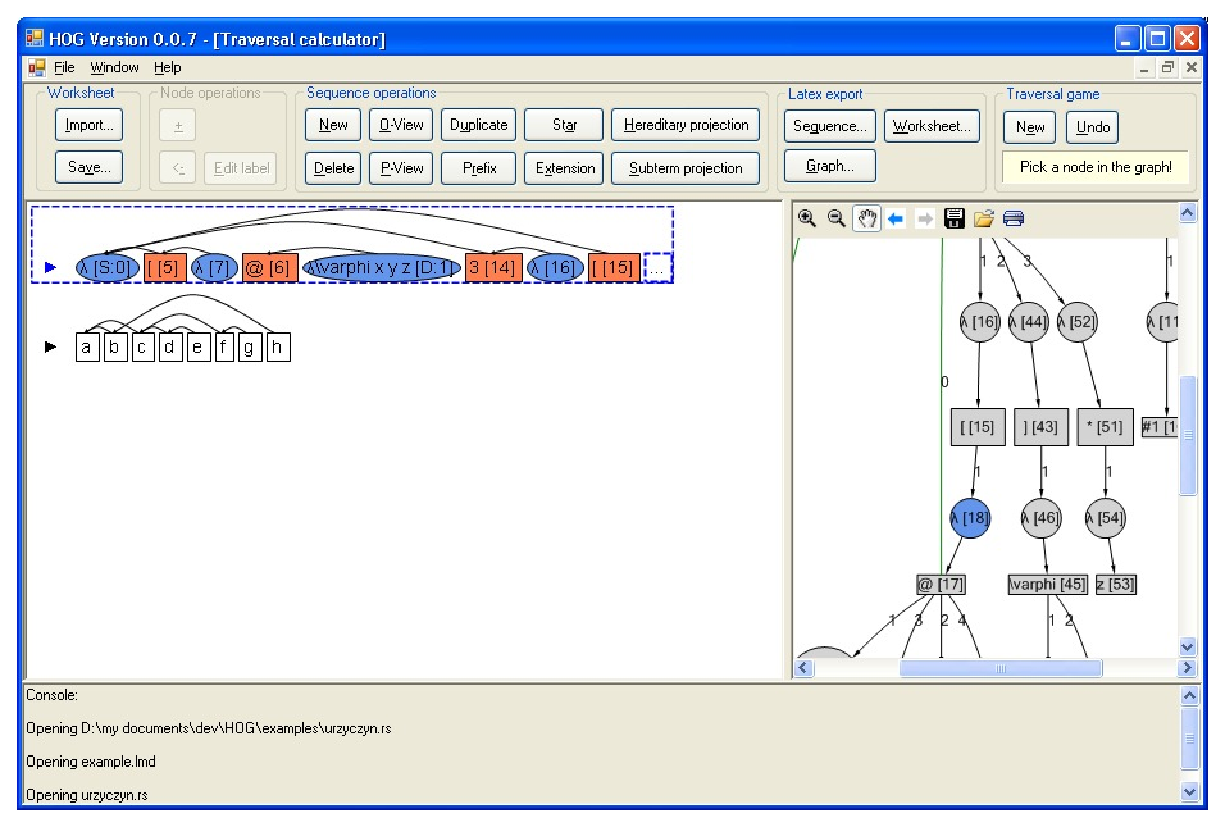
\includegraphics[width=15cm]{sshot_traversal}\\
\end{bigcenter}
  \caption{Screenshot of a traversal game in \toolname.}
  \label{fig:sshot_hog_traversal}
\end{figure}

The right-hand side of the window contains a representation of the computation graph and the left part of the window contains a list of justified sequences created by the user. In the screenshot, the first justified sequence corresponds to a traversal that is being played by the user. Opponent moves and Proponent moves are represented by circles and rectangular nodes respectively. The user make a move by selecting a node among the valid nodes highlighted in the computation graph. If there is a unique possible
 justifier in the traversal then the move is automatically
accepted, otherwise the user has to specify a move by selecting a valid justifier in the traversal. After the move is accepted \toolname\ responds with a P-move. This goes on until the traversal is maximal.

\toolname\ allows the user to perform several operations on the justified sequence such as computing the P-view or the O-view. It is also possible to export the sequence to \LaTeX\ code. For example, typesetting the traversal from Figure \ref{fig:sshot_hog_traversal} with \LaTeX\ produces
$$\Pstr[0.7cm]{(n0){\lambda }\ (n1-n0){[}\ (n2-n1){\lambda }\ (n3){@}\ (n4-n3){\lambda \varphi x y z}\ (n5-n0){3}\ (n6-n5){\lambda }\ (n7-n0){[}\ {...}\ }$$

\subsection{Other features}




\subsubsection{Generating a CPDA from a recursion scheme}
\toolname\ can  convert any higher-order recursion scheme into an equivalent (\ie generating the same infinite tree) Collapsible Push-down Automaton (CPDA) of the same order. The algorithm used to perform this transformation is taken from \cite{hague-sto07}.

The transition function of a CPDA is given by a list of instructions which we call the ``code'' of the CPDA. Figure \ref{fig:cpda_listing} give an example of CPDA generated from the Urzyczin recursion scheme.

\begin{figure}
\begin{lstlisting}[breaklines=true,basicstyle=\tiny]
Order: 2

Stack alphabet: 0 1 2 3 4 5 6 7 8 9 10 11 12 13 14 15 16 17 18 19 20 21 22 23 24 25 26 27 28 29 30 31 32 33 34 35 36 37 38 39 40 41 42 43 44 45 46 47 48 49 50 51 52 53 54 55 56 57 58 59

Code:
Code:

    0                   PUSH1 0 (0,0)
    1 start          :  CASETOP0 0->NODE0 1->NODE1 2->NODE2 3->NODE3 4->NODE4 5->NODE5 6->NODE6 7->NODE7 8->NODE8 9->NODE9 10->NODE10 11->NODE11 12->NODE12 13->NODE13 14->NODE14 15->NODE15 16->NODE16 17->NODE17 18->NODE18 19->NODE19 20->NODE20 21->NODE21 22->NODE22 23->NODE23 24->NODE24 25->NODE25 26->NODE26 27->NODE27 28->NODE28 29->NODE29 30->NODE30 31->NODE31 32->NODE32 33->NODE33 34->NODE34 35->NODE35 36->NODE36 37->NODE37 38->NODE38 39->NODE39 40->NODE40 41->NODE41 42->NODE42 43->NODE43 44->NODE44 45->NODE45 46->NODE46 47->NODE47 48->NODE48 49->NODE49 50->NODE50 51->NODE51 52->NODE52 53->NODE53 54->NODE54 55->NODE55 56->NODE56 57->NODE57 58->NODE58 59->NODE59
    2 NODE0          :  PUSH1 5 (1,1)
    3                   GOTO start
    4 NODE1          :  PUSH1 14 (1,1)
    5                   GOTO start
    6 NODE2          :  PUSH1 55 (1,1)
    7                   GOTO start
    8 NODE3          :  PUSH1 58 (1,1)
    9                   GOTO start
   10 NODE4          :  PUSH1 59 (1,1)
   11                   GOTO start
   12 NODE5          :  EMIT [ NODE5_1
   13 NODE5_1        :  PUSH1 7 (0,0)
   14                   GOTO start
   15 NODE6          :  PUSH1 1 (1,1)
   16                   GOTO start
   17 NODE7          :  PUSH1 6 (1,1)
   18                   GOTO start
   19 NODE8          :  PUSH1 4 (1,1)
   20                   GOTO start
   21 NODE9          :  PUSH1 8 (1,1)
   22                   GOTO start
   23 NODE10         :  REPEAT 3 TIMES POP1
   24                   COLLAPSE
   25                   CASETOP0 45->NODE10_45 21->NODE10_21
   26                   FAILWITH "Unexpected top 0-element!"
   27 NODE10_21      :  PUSH1 24 (3,1)
   28                   GOTO start
  ...
\end{lstlisting}
\label{fig:cpda_listing}
\caption{Excerpt of the listing of the CPDA generated  from the Urzyczin recursion scheme.}
\end{figure}

A line of code of the CPDA is made of three parts: the line number, an optional label and an instruction. There are four kinds of instructions: stack instructions, the node emitting instruction, branching instructions and debugging instructions. The stack instructions are:
\begin{description}
  \item[{\tt PUSH1 a (j,k)}] push the element {\tt a} on the top 1-stack an associates the link $(j,k)$ to it. This encoding means that the link points to a prefix stack obtained by performing an order-$j$ pop $k$ consecutive times.
  \item[{\tt PUSHn}] performs an order $n$ push on the stack (duplicates the top $n-1$-stack).
  \item[{\tt POPn}] performs an order $n$ pop on the stack (pop the top $n-1$-stack).
  \item[{\tt COLLAPSE}] collapses the stack to the prefix stack pointed to by the top element in the stack. In other words it executes $k$ times the execution {\tt POPj} where {\tt (j,k)} is the encoding of the link associated to the top element.

  \item[{\tt REPEAT n TIMES ins}] repeats the instruction {\tt ins} $n$ times where $n$ is a constant. The behaviour is unspecified if {\tt ins} is a branching instruction.
\end{description}

In order to create nodes in the value-tree, the CPDA uses teh following special instruction:
\begin{description}
  \item[$\mathtt{EMIT\ f\ LAB_1 \ldots LAB_k}$] emits the terminal $f$ of type $o^k \rightarrow o$.
   The CPDA is then spawn into $k$ other CPDA's, one for each parameter of the terminal $f$.
   The $i's$ spawn CPDA will be started at instruction $\mathtt{LAB_i}$ for $i \in \{1..k\}$.
\end{description}

The branching instructions are:
\begin{description}
  \item[{\tt GOTO lab}] jumps to the label {\tt lab}.
  \item[$\mathtt{CASTOP0\ e_0->lab_0 ... e_k->lab_k}$] performs a test case on the element
  at the top of the stack. If the top element is equal to $\mathtt{e_i}$ for some $i \in \{0..k\}$
  then the CPDA jumps to the label $\mathtt{lab_k}$. Otherwise it moves on to the following instruction.
\end{description}

There are also instructions used for debugging the code of a CPDA:
\begin{description}
  \item[{\tt FAILWITH msg}] raises an exception with the message {\tt msg}.
  \item[{\tt ASSERT msg}] asserts that the condition described by the message {\tt msg} is verified. If the test fails then an exception is raised.
\end{description}



A configuration of the CPDA is given by an instruction number together with an order-$n$ stack. In the initial configuration, the CPDA is positioned on the first instruction and the stack is the empty order-$n$ stack. After executing a transition the CPDA moves to the next instruction (or jump to another line if it is a branching instruction).




\subsubsection{Exploring the value tree by executing the CPDA transitions }

When you open a CPDA, \toolname\ displays a lazy value tree (Figure \ref{fig:sshot_cpda}). Each node of this tree corresponds to a configuration of the CPDA. Nodes are either labelled by an instruction number or by a terminal. In a separate textbox, \toolname\ shows the content of the stack for the selected configuration.

\begin{figure}
\begin{bigcenter}
  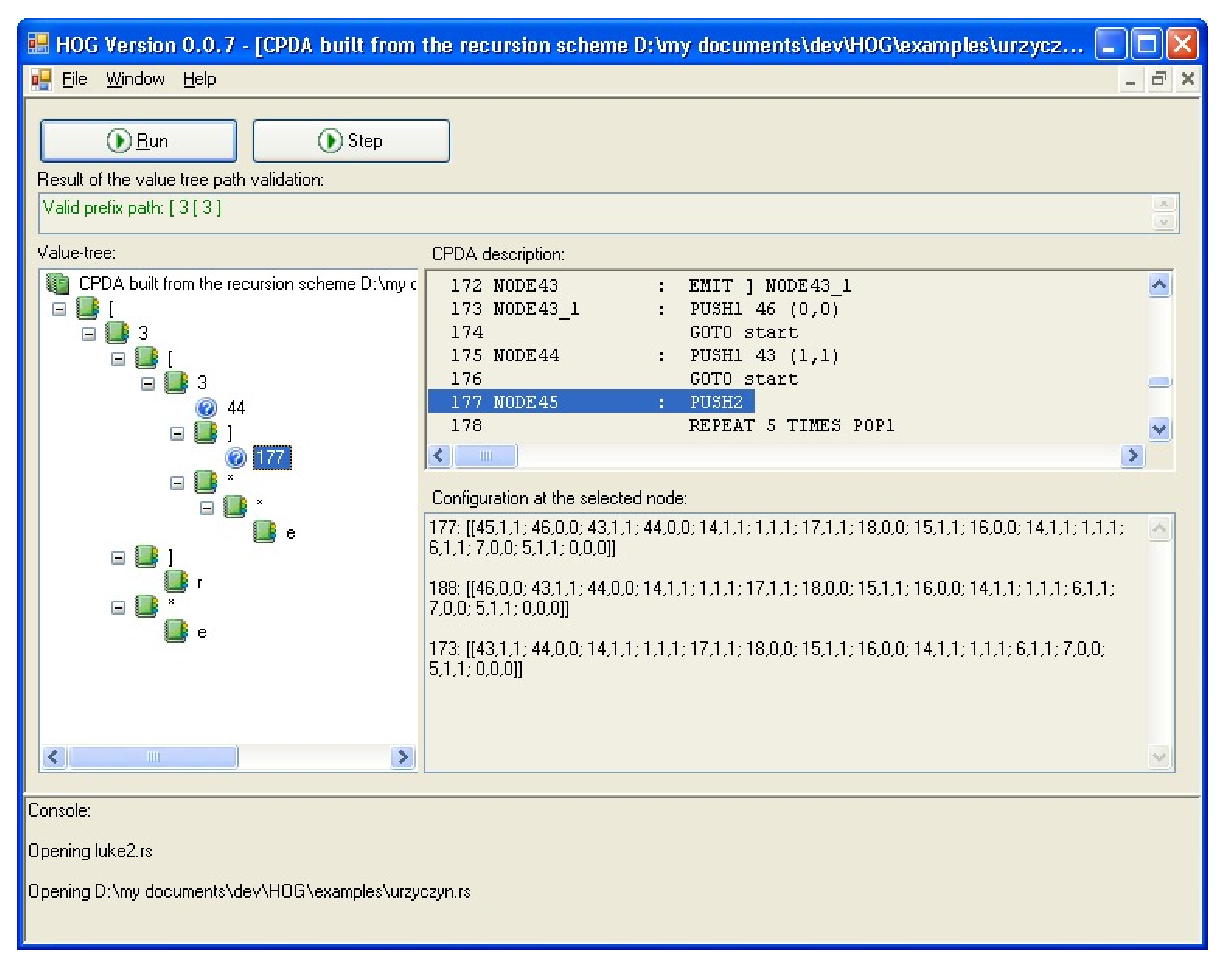
\includegraphics[width=14cm]{sshot_cpda}\\
\end{bigcenter}
  \caption{\toolname\ executing the CPDA generated from the Urzyczin recursion scheme.}
  \label{fig:sshot_cpda}
\end{figure}

Initially, the root node is labeled with the instruction number $0$ which corresponds to the first instruction of the CPDA code. When executing the CPDA transition on a node, the stack is updated accordingly and the node label is updated to the next instruction to be executed. This process is repeated until reaching an {\tt EMIT} instruction.

When an instruction $\mathtt{EMIT\ f\ LAB_1 \ldots LAB_k}$ is executed (which means that a terminal $f:o^k\rightarrow o$ is emitted), a node labelled $f$ is created in the value tree with $k$ children nodes are attached to it. Each child corresponds to a newly spawn CPDA with the same stack as in the original configuration. Finally, the current instruction of the  $i$th child is set to the instruction number with label $\mathtt{LAB_i}$.

Terminal nodes represent the actual nodes of the value-tree and as such cannot be expanded further.

\subsubsection{Exploring the tree generated by a recursion scheme}

\toolname\ has another feature which allows one to explore the infinite tree generated from a given recursion scheme without the need to convert it into a CPDA beforehand.


    \bibliographystyle{plain}
    \bibliography{../bib/dphil-all}

\end{document}

\usepackage{graphicx}
\usepackage{url}
\def\toolname{HOG}


\title{A tool illustrating the Correspondence Theorem
\\ GALOP 2008}

\author{William~Blum~~~~~~~~~~~C.-H.~Luke~Ong\\
Oxford University Computing Laboratory\\
Wolfson Building, Parks Road, Oxford OX1 3QD, ENGLAND\\
\{william.blum,luke.ong\}@comlab.ox.ac.uk }



\begin{document}
\maketitle \thispagestyle{empty}

\begin{abstract}
Todo...
\end{abstract}

\tableofcontents

\section{Luke's description of the paper:}

 We have developed a number of what we call Path-Traversal
Correspondence Theorems. One way to think of the work is as a kind of representation theory of the game semantics of higher-type programs (such as recursion schemes, PCF and Idealized Algol) that is very concrete, involving combinatorics over (possibly) infinite structures defined by the abstract syntax trees of the programs being modelled. The idea is that we represent a play in the strategy-denotation of a term as the underlying "hereditarily uncovered" interaction sequence, called traversal. Another way to put it is that traversals are built up by performing parallel-composition but WITHOUT the hiding. This is what William Greenland has called (in his thesis) "revealed semantics" (or "interaction semantics"). A consequence of the representation is that we show how the "innocent game" given by a term can be played out very concretely over what is in essence the abstract syntax tree of the term itself.

This "representation theory" was first developed to prove the result in my LICS06 paper (i.e. trees generated by higher-order recursion schemes have decidable MSO theories). The theory has at least two other applications. First as a justification of the game characterization of the Higher-Order Matching Problem (but NOT the algorithm) developed by Colin Stirling, and secondly as a key lemma underpinning the result that
 the following are equivalent (i.e. equi-expressive:
i. order-n recursion schemes (= order-n PCF terms generated from uninterpreted order-1 symbols) ii. order-n collapsible pushdown automata CPDA. iii. order-n "pure" innocent strategies

What we are thinking of submitting is a short paper describing a tool developed by William Blum that illustrates the representation theory. The tool has many capabilities. For example, it can perform the inter-translation between CPDA and recursion schemes; it can demonstrate the path-traversal correspondence in the form of a 2-player game (and lets users play it out over the abstract syntax tree of the term); and it is a very impressive tool for drawing justified sequences!

What we intend to talk about in the paper is first an overview of the correspondence theorems, illustrate their many applications, and then showcase the tool.

\section{Computation tree, Traversals and the Correspondence Theorem}

In \cite{OngLics2006}, one of us introduced the notion of computation tree and traversals over a computation tree for the purpose of studying trees generated by higher-order recursion scheme. Here we extend these concepts to the pure (\ie without constants) simply-typed lambda calculus. Our setting allows the presence of free variable of any order. Moreover the term studied is not necessarily of ground type. (This contrasts with \cite{OngLics2006}'s setting where the term is of ground type and contains only \emph{uninterpreted constant}\footnote{A constant $f$ is  \emph{uninterpreted} if the small-step semantics of the language
  does not contain any rule of the form $f \dots \rightarrow e$. $f$
  can be regarded as a data constructor.} of order 1 at most and no
free variables.) Note that our setting automatically accounts for the presence of uninterpreted constants since they can be regarded as free variables. We will then state the \emph{Correspondence Theorem} (Theorem \ref{thm:correspondence}).

In the following we fix a simply-typed term $\Gamma \vdash M :T$.

\subsection{Computation tree}
 In \cite{OngLics2006} the computation tree of a grammar is
defined as the unravelling of a finite graph representing the long transform of a grammar. Similarly we define the computation tree of a $\lambda$-term as an abstract syntax tree of its $\eta$-long normal form.  We write $l\langle t_1, \ldots, t_n \rangle$ with $n \geq 0$ to denote the tree with a root labelled $l$ with $n$ children subtrees $t_1$, \ldots, $t_n$.

\begin{definition}\rm
\label{dfn:comptree}
  The \defname{computation tree} $\tau(M)$ of a simply-typed term
  $\Gamma \vdash M:T$ with variable names in a countable set
  $\mathcal{V}$ is a tree with labels in $ \{ @ \} \union \mathcal{V}
  \union \{ \lambda x_1 \ldots x_n \ | \ x_1 ,\ldots, x_n \in
  \mathcal{V}, n\in\nat \}$ defined from its $\eta$-long form as follows.
  Let $\overline{x}$ denote some list of variables $x_1 \ldots x_n$ for some $n\geq 0$.
\begin{eqnarray*}
  \mbox{For $m\geq 0$, $z \in \mathcal{V}$: } \tau(\lambda \overline{x} . z s_1 \ldots s_m ) &=& \lambda \overline{x} \langle z \langle\tau(s_1),\ldots,\tau(s_m)\rangle\rangle \\
  \mbox{For $m \geq 1$: } \tau(\lambda \overline{x} . (\lambda y.t) s_1 \ldots s_m) &=& \lambda \overline{x} \langle @ \langle \tau(\lambda y.t),\tau(s_1),\ldots,\tau(s_m) \rangle \rangle \ .
\end{eqnarray*}
\end{definition}

Even-level nodes are $\lambda$-nodes (the root is on level 0). A single $\lambda$-node can represent several consecutive variable abstractions or it can just be a \emph{dummy lambda} if the corresponding subterm is of ground type.  Odd-level nodes are variable or application nodes.

We say that a variable node $n$ labelled $x$ is \defname{bound} by a node $m$, and $m$ is called the \defname{binder} of $n$, if $m$ is the closest node in the path from $n$ to the root such that $m$ is labelled $\lambda \overline{\xi}$ with $x\in \overline{\xi}$.


We write $\theroot$ to denote the root of the computation tree $\tau(M)$. The set of nodes of the computation tree is denoted by $N$. The sets $N_@$, $N_\lambda$ and $N_{\sf var}$ are the subset of $N$ consisting of the @-nodes, $\lambda$-nodes and variable nodes respectively.


\subsection{Justified sequences of nodes}

We define the \defname{enabling relation} on the set of nodes of the computation tree as follows: $m$ enables $n$, written $m \vdash n$, if and only if $n$ is bound by $m$ (and we sometimes write $m \vdash_i n$ to precise that $n$ is the $i^{\sf th}$ variable bound by $m$); or $m$ is the root $\theroot$ and $n$ is a free variable; or $n$ is a $\lambda$-node and $m$ is its parent node.


We say that a node $n_0$ of the computation tree is
\defname{hereditarily enabled} by $n_p \in N$ if there are nodes
$n_1,\ldots, n_{p-1} \in N$ such that $n_{i+1}$ enables $n_{i}$ for all $i\in 0..p-1$.

For any set of nodes $S, H \subseteq N$ we write $S^{H\vdash}$ for $S \inter \vdash^*(H) = \{ n \in S \ | \exists n_0 \in H \mbox{ s.t. }n_0  \vdash^* n \}$ -- the subset of $S$ constituted of nodes hereditarily enabled by some node in $H$. We will abbreviate $S^{\{n_0\}\vdash}$ into $S^{n_0\vdash}$.

We call \defname{input-variables nodes} the elements of $V_{\sf var}^{\theroot\vdash}$ \ie variables that are hereditarily enabled by the root of $\tau(M)$. Thus we have $V_{\sf var}^{\theroot\vdash} = V \setminus ( V_{\sf var}^{N_@\vdash} \union V_{\sf var}^{N_\Sigma\vdash})$.

A \defname{justified sequence of nodes} is a sequence of nodes with pointers such that each occurrence of a variable or $\lambda$-node $n$ different from the root has a pointer to some preceding occurrence $m$ verifying $m \vdash n$. In particular, occurrences of @-nodes do not have pointer. We represent the pointer in the sequence as follows \Pstr[0.4cm]{ (m){m} \ldots (n-m,45:i) n }.
 where the label indicates that either $n$ is labelled with the $i$th variable
abstracted by the $\lambda$-node $m$ or that $n$ is the $i^{\sf th}$ child of $m$.  Children nodes are numbered from $1$ onward except for @-nodes where it starts from $0$. Abstracted variables are numbered from $1$ onward. The $i^{\sf th}$ child of $n$ is denoted by $n.i$.

We say that a node $n_0$ of a justified sequence is
\defname{hereditarily justified} by $n_p$ if there are occurrences $n_1,
\ldots, n_{p-1}$ in the sequence such that $n_i$ points to $n_{i+1}$ for all $i\in 0..p-1$. Let $n$ be an occurrence in a justified sequence $s$. We write $s \filter r$ to denote the subsequence of $s$ consisting of the occurrences hereditarily justified by $n$.


The notion of \defname{P-view} $\pview{t}$ of a justified sequence of nodes $t$ is defined the same way as the P-view of a justified sequences of moves in Game Semantics:\footnote{ The equalities in the
  definition determine pointers implicitly. For instance in the second
  clause, if in the left-hand side, $n$ points to some node in $s$
  that is also present in $\pview{s}$ then in the right-hand side, $n$
  points to that occurrence of the node in $\pview{s}$.}
$$\begin{array}{rclrcl}
\pview{\epsilon} &=&  \epsilon & \pview{\Pstr[0.5cm]{ s \cdot (m) m \cdot \ldots \cdot (lmd-m,40){\lambda\overline{\xi}} }}
 &=& \Pstr{
\pview{s} \cdot (m2) m \cdot (lm2-m2,50) {\lambda \overline{\xi}} } \\
\mbox{for $n \notin N_\lambda$, } \pview{s \cdot n }  &=&  \pview{s} \cdot n \qquad & \pview{s \cdot \theroot }  &=&  \theroot
\end{array}$$

The O-view of $s$, written $\oview{s}$, is defined dually. We will borrow the game semantic terminology: A justified sequences of nodes satisfies \defname{alternation} if for any two consecutive nodes one is a $\lambda$-node and the other is not, and \defname{P-visibility} if every variable node points to a node occurring in the P-view a that point.

\subsection{Adding value-leaves to the computation tree}

We now add another ingredient to the computation tree that was not originally used in \cite{OngLics2006}.  We write $\mathcal{D}$ to denote the set of values of the base type $o$.  We add
\defname{value-leaves} to $\tau(M)$ as follows: For each value $v
\in \mathcal{D}$ and for each node $n \in N$ we attach the child leaf $v_n$ to $n$.  We write $V$ for the set of vertices of the resulting tree (\ie inner nodes and leaf nodes). For $\$$ ranging in $\{@, \lambda, var \}$, we write $V_\$$ to denote the set of inner nodes from $N_\$$ plus the leaf-nodes whose parent is in $N_\$$ \ie $V_\$ = N_\$ \union \{ v_n \ | \ n \in N_\$, v \in \mathcal{D} \}$.


Everything that we have defined can be lifted to this new version of computation tree. The enabling relation $\vdash$ is extended so that every leaf is enabled by its parent node. A link going from a value-leaf $v_n$ to a node $n$ is labelled by $v$: \Pstr[0.4cm]{ (n) n \ldots (vn-n,35:v){v_n} }. For the definition of P-view and visibility, value-leaves are treated as $\lambda$-nodes if they are at an odd level in the computation tree, and as variable nodes if they are at an even level.

We say that an occurrence of an inner node $n \in N$ is
\defname{answered} by an occurrence $v_n$ if $v_n$ in
the sequence that points to $n$, otherwise we say that $n$ is
\defname{unanswered}. The last unanswered node is called the
\defname{pending node}.  A justified sequence of nodes is
\defname{well-bracketed} if each value-leaf occurring in it is justified by the pending node at that point.  If $t$ is a traversal then we write
$?(t)$ to denote the subsequence of $t$ consisting only of unanswered nodes.

\subsection{Traversals of the computation tree}
\label{subsec:traversal}

A \emph{traversal} is a justified sequence of nodes of the computation tree where each node indicates a step that is taken during the evaluation of the term.

\begin{definition}[Traversals for simply-typed $\lambda$-terms] \rm
\label{def:traversal} The set $\travset(M)$ of \defname{traversals}
over $\tau(M)$ is defined by induction over the rules of Table
\ref{tab:trav_rules}. A traversal that cannot be extended by any
rule is said to be \emph{maximal}.
\end{definition}

\begin{FramedTable}
\noindent {\bf Initialization rules}
\begin{itemize}[]
\item\rulenamet{Empty} $\epsilon \in \travset(M)$.
\item\rulenamet{Root} The sequence constituted of a single occurrence of $\tau(M)$'s root is a traversal.
\end{itemize}

\noindent {\bf Structural rules}
\begin{itemize}[]
    \item \rulenamet{Lam} If $t \cdot \lambda \overline{\xi}$ is a traversal then so is
        $t \cdot \lambda \overline{\xi} \cdot n$ where $n$
        denotes $\lambda \overline{\xi}$'s child and:
        \begin{compactitem}
            \item If $n \in N_@ \union N_\Sigma$ then it has no justifier;
            \item if  $n \in N_{\sf var}\setminus N_{\sf fv}$ then it points to the only occurrence\footnote{Prop.\ \ref{prop:pviewtrav_is_path} will show that P-views
            are paths in the tree thus $n$'s enabler occurs
            exactly once in the P-view.} of its binder in
            $\pview{t\cdot \lambda \overline{\xi}}$;
            \item if  $n \in N_{\sf fv}$ then it points
            to the only occurrence of the root $\theroot$ in
            $\pview{t \cdot \lambda \overline{\xi}}$.
        \end{compactitem}
    \item \rulenamet{App} If $t \cdot @$ is a traversal then so is \Pstr[0.4cm]{t \cdot (m) @  \cdot (n-m,40:0) n}.
\end{itemize}

\emph{\bf Input-variable rules}
\begin{itemize}[]
\item \rulenamet{InputVar} If $t$ is a traversal where $t^\omega \in N_{\sf var}^{\theroot\vdash} \union L_\lambda^{\theroot\vdash}$
and $x$ is an occurrence of a variable node in $\oview{t}$ then
so is $t \cdot n$ for any child $\lambda$-node $n$ of $x$, $n$
pointing to $x$.



\item \rulenamet{InputValue} If $t_1
\cdot x \cdot t_2$ is a traversal with pending node $x \in
N_{\sf var}^{\theroot\vdash}$ then so is \Pstr[0.5cm]{t_1 \cdot
(x){x} \cdot t_2 \cdot (xv-x,38:v){v_x} } for all $v \in
\mathcal{D}$.
\end{itemize}

\emph{\bf Copy-cat rules}
\begin{itemize}[]
\item\rulenamet{Var}
If \Pstr[0.5cm]{t \cdot (n){n} \cdot (lx){\lambda \overline{x}}
    \ldots (x-lx,50:i){x_i} } is a traversal where $x_i \in
    N_{\sf var}^{@\vdash}$ then so is \Pstr[0.5cm]{ t \cdot
(n){n} \cdot (lx){\lambda \overline{x}}  \ldots (x-lx,30:i){x_i}
    \cdot (letai-n,40:i){\lambda \overline{\eta_i}}
     }.

\item\rulenamet{Value}
  If \Pstr{t \cdot (m){m} \cdot (n){n}  \ldots
(vn-n,60:v){v}_{n} } is a traversal where $n\in N$ then so is
\Pstr[0.6cm]{t \cdot (m){m} \cdot (n){n} \ldots
(vn-n,60:v){v}_{n} \cdot (vm-m,45:v){v}_m}.
\end{itemize}
\caption[Traversal rules for the simply-typed
lambda-calculus]{Traversal rules for the simply-typed
$\lambda$-calculus.}
 \label{tab:trav_rules}
\end{FramedTable}


\parpic[r]{
 $\pssetcomptree\tree[levelsep=3ex,treesep=0.5cm]{\lambda} {
    \tree{@}{
        \pstree[linestyle=dotted]{\TR{\lambda y}\arclabel{0} }{
            \tree{y}{
                \tree{\lambda \overline{\eta_1}}{\vdots}%\arclabel{1}
                \tree{\lambda \overline{\eta_i}}{\vdots}%\arclabel{i}
                \tree{\lambda \overline{\eta_n}}{\vdots}%\arclabel{n}
            }
        }
        \pstree[linestyle=dotted]{\TR{\lambda \overline{x}}
            \arclabel{1}}{ \tree{x_i}{\TR{} \TR{}}}
}}$ } A traversal always starts by visiting the root. Then it mainly follows the structure of the tree. The (Var) rule permits to jump across the computation tree. The idea is that after visiting a variable node $x$, a jump is allowed to the node corresponding to the subterm that would be substituted for $x$ if all the $\beta$-redexes occurring in the term were reduced. The sequence \Pstr[0.8cm]{\lambda \cdot (app) @  \cdot (ly) {\lambda y}  \ldots (y-ly,35:1) y  \cdot (lx-app,38:1) {\lambda \overline{x}} \ldots (x-lx,30:i) {x_i} \cdot (leta-y,40:i) {\lambda \overline{\eta_i} } \ldots}
 is an example of traversal of the computation tree shown on the right.

\begin{proposition}[counterpart of proposition 6 from \cite{OngHoMchecking2006}]
\label{prop:pviewtrav_is_path} Let $t$ be a traversal. Then:
\begin{enumerate}[(i)]
\item $t$ is a well-defined and well-bracketed justified sequence;
\item $t$ is a well-defined justified sequence verifying alternation, P-visibility and O-visibility;
\item If $t$'s last node is not a value-leaf, then $\pview{t}$ is the path in the computation tree going from the root to $t$'s last node.
\end{enumerate}
\end{proposition}

The \defname{reduction} of a traversal $t$ is the subsequence of $t$ obtained by keeping only occurrences of nodes that are hereditarily enabled by the root $\theroot$. This has the effect of eliminating the ``internal nodes'' of the computation. If $t$ is a non-empty traversal then the root $\theroot$ occurs exactly once in $t$ and the reduction of $t$ is equal to $t \filter r$. We write $\travset(M)^{\filter \theroot}$ for the set or reduction of traversals of $M$.

Application nodes are used to connect the operator and the operand of an application in the computation tree but since they do not play any role in the computation of the term, we can remove them from the traversals.  We write $t-@$ for the sequence of nodes-with-pointers obtained by removing from $t$ all @-nodes and value-leaves of @-nodes, any link pointing to an @-node being replaced by a link pointing to the immediate predecessor of @ in $t$. We write $\travset(M)^{-@}$ for the set $\{ t - @ \ | \  t \in \travset(M) \}$.
\begin{remark}
If $M$ is $\beta$-normal then $\tau$ does not contain any @-node therefore all nodes are hereditarily justified by $r$ and we have $\travset(M)^{-@} = \travset(M) = \travset(M)^{\filter \theroot }$.
\end{remark}

\subsection{Revealed Game Semantics}

In game semantics, strategy composition is achieved by performing a CSP-like ``composition + hiding''. If the internal moves are not hidden then we obtain an alternative semantics called \emph{revealed semantics} in \cite{willgreenlandthesis} and \emph{interaction} semantics in \cite{DBLP:conf/sas/DimovskiGL05}. Here we will refer to this semantics as the \defname{fully revealed game semantics}. The fully revealed game denotation of a term $\Gamma \vdash M :T$, written $\revsem{\Gamma \vdash M : T}$, is obtained by uncovering\footnote{An algorithm that uniquely recovers hidden moves is given in Part II of
  \cite{hylandong_pcf}.} all the internal moves from $\sem{\Gamma \vdash
  M : T}$ generated during strategy composition.
We introduce a variation of the fully-revealed game denotation called the \defname{syntactically-revealed game denotation}, written $\syntrevsem{\Gamma \vdash
  M : T}$. In this denotation, as opposed to the fully-revealed denotation,
only \emph{certain} internal moves from $\sem{\Gamma \vdash
  M : T}$ are uncovered: The internal moves that are generated by the composition with the evaluation map
$ev$ at a @-node of the computation tree are all uncovered, but in the denotation of a subtem of the form $y N_1 \ldots N_p$ for some $p\geq1$, only certain internal moves are uncovered. The formal definition can be found in \cite{localbeta2008}.

\subsection{Computation trees and arenas}
We consider the well-bracketed game model of the simply-typed lambda calculus.  We choose to represent strategies using ``prefix-closed set of plays''. \footnote{In the literature, a strategy is usually defined as a set of plays closed by \emph{even}-length prefix. For the purpose of showing the Correspondence Theorem, however, the ``prefix-closed''-based definition is more adequate.} We fix a term $\Gamma \vdash M : T$ and write $\sem{\Gamma \vdash M : T}$ for its strategy denotation. The answer moves of a question $q$ are written $v_q$ where $v$ ranges in $\mathcal{D}$.

\begin{proposition}
There exists a function $\varphi_M$, constructible from $\tau(M)$, that maps nodes from $V\setminus (V_@ \union V_\Sigma)$ to moves of the interaction arena underlying the revealed strategy $\syntrevsem{\Gamma \vdash M : T}$ and such that $\varphi$ maps $\lambda$-nodes to O-questions, variable nodes to P-questions, value-leaves of $\lambda$-nodes to P-answers and value-leaves of variable nodes to O-answers.
\end{proposition}

\begin{example}
Take $\lambda x . (\lambda g . g x) (\lambda y . y)$ with $x,y:o$ and $g:(o,o)$. The diagram below represents the computation tree (middle), the arenas $\sem{(o,o), o}$ (left), $\sem{o , o}$ (right), $\sem{o\rightarrow o}$ (rightmost) and $\varphi = \psi \union \psi_{\lambda g.g x}^{\lambda g, q_{\lambda g}} \union \psi_{\lambda y.y}^{\lambda y, q_{\lambda y}}$ (dashed-lines).
$$\psset{levelsep=3.5ex}
\pstree{\TR[name=root]{\lambda x}} {
    \pstree{\TR[name=App]{@}}
    {
            \pstree{\TR[name=lg]{\lambda g}}
                { \pstree{\TR[name=lgg]{g}}{
                        \pstree{\TR[name=lgg1]{\lambda}}
                        { \TR[name=lgg1x]{x}  } } }
            \pstree{\TR[name=ly]{\lambda y}}
                    {\TR[name=lyy]{y}}
    }
} \rput(4.5cm,-1cm){
  \pstree{\TR[name=A1lx]{q_{\lambda x}}}
        { \TR[name=A1x]{q_x} }
} \rput(-6cm,-1.5cm){
    \pstree{\TR[name=A2lg]{q_{\lambda g}}}
    {
        \pstree{\TR[name=A2g]{q_g}}
        {  \TR[name=A2g1]{q_{g_1}}   }
    }}
\rput(2.5cm,-1.5cm){
    \pstree{\TR[name=A3ly]{q_{\lambda y}}}
        { \TR[name=A3y]{q_y}
        }
} \psset{nodesep=1pt,arrows=->,arcangle=-20,arrowsize=2pt 1,linestyle=dashed,linewidth=0.3pt} \ncline{->}{root}{A1lx} \mput*{\psi} \ncarc{->}{lgg1x}{A1x} \ncline{->}{lg}{A2lg} \mput*{\psi_{\lambda g.g x}^{\lambda g, q_{\lambda g}}} \ncline{->}{lgg}{A2g} \ncline{->}{lgg1}{A2g1} \ncline{->}{ly}{A3ly} \mput*{\psi_{\lambda y.y}^{\lambda y, q_{\lambda y}}} \ncline{->}{lyy}{A3y}
$$
\end{example}

We extend the function $\varphi$ to justified sequences of nodes as follows: If $t = t_0 t_1 \ldots$ is a justified sequence of nodes in $V_\lambda \union V_{\sf var}$ then $\varphi(t)$ is defined to be the sequence of moves $\varphi(t_0)\ \varphi(t_1) \ldots$ equipped with the pointers of $t$.


\subsection{The Correspondence Theorem}


In the simply-typed lambda calculus, the set $\travset(M)$ of traversals of the computation tree is isomorphic to the set of plays of the syntactically-revealed denotation. Moreover the set of traversal reductions is isomorphic to the standard strategy denotation:

\begin{theorem}[The Correspondence Theorem]
\label{thm:correspondence} The function $\varphi_M$ gives us the following two isomorphisms:
\begin{eqnarray*}
(i)~\varphi_M  &: \travset(M)^{-@} \stackrel{\cong}{\longrightarrow} \syntrevsem{\Gamma \vdash M :T} \\
(ii)~\varphi_M  &: \travset(M )^{\filter \theroot} \stackrel{\cong}{\longrightarrow} \sem{\Gamma \vdash M : T} \ .
\end{eqnarray*}
\end{theorem}

\begin{example}
Take $M = \lambda f z . (\lambda g x . f x) (\lambda y. y) (f z) : ((o,o),o, o)$.  The figure below represents the computation tree (left tree), the arena $\sem{((o,o),o, o)}$ (right tree) and $\psi_M$ (dashed line). (Only question moves are shown for clarity.) The justified sequence of nodes $t$ defined hereunder is an example of traversal:

\begin{tabular*}{\textwidth}{lcp{6.3cm}}
$\pssetcomptree\pstree[levelsep=2.5ex,treesep=0.3cm]{ \TR[name=root]{\lambda f z} }
     {  \tree[levelsep=4ex]{@}
        {   \tree{\lambda g x}{
                  \pstree{\TR[name=f]{f^{[1]}}}{
                            \pstree{\TR[name=lmd]{\lambda^{[2]}}}
                                {\TR{x}}
                  }
                }
            \tree{\lambda y }{\TR{y}}
            \tree{\lambda ^{[3]}}{
                \pstree{\TR[name=f2]{f^{[4]}}} {
                \pstree{\TR[name=lmd2]{\lambda^{[5]}}}{\TR[name=z]{z}}
                }
            }
        }
     }
\hspace{1cm}
  \pstree[levelsep=8ex, treesep=0.3cm]{ \TR[name=q0]{q^0} }
    {   \pstree[levelsep=4ex]{\TR[name=q1]{q^1}} {\TR[name=q2]{q^2}}
        \TR[name=q3]{q^3}
    }
\psset{nodesep=1pt,arrows=->,arrowsize=2pt 1,linestyle=dashed,linewidth=0.3pt} \ncline{->}{root}{q0} \mput*{\psi_M} \ncarc[arcangle=-25]{->}{z}{q3} \ncarc[arcangle=10]{->}{f}{q1} \ncarc[arcangle=10]{->}{lmd}{q2} \ncline{->}{f2}{q1} \ncline{->}{lmd2}{q2}$ &  &
\begin{asparablank}
  \item  \Pstr[0.8cm]{
t = (n){\lambda f z} \ (n2){@} \ (n3-n2,60){\lambda g x} \ (n4-n,45){f^{[1]}} \ (n5-n4,45){\lambda^{[2]}} \ (n6-n3,45){x} \ (n7-n2,35){\lambda^{[3]}} \ (n8-n,35){f^{[4]}} \ (n9-n8,45){\lambda^{[5]}} \ (n10-n,35){z} }

\item \Pstr[0.9cm]{
t\filter r = (n){\lambda f z} \ (n4-n,50){f}^{[1]} \ (n5-n4,60){\lambda}^{[2]} \ (n8-n,45){f}^{[4]} \ (n9-n8,60){\lambda}^{[5]} \ (n10-n,40){z}}
\item
\Pstr[0.8cm]{ {\varphi_M(t\filter r) =\ } (n){q^0}\ (n4-n,60){q^1}\ (n5-n4,60){q^2}\ (n8-n,45){q^1}\ (n9-n8,60){q^2}\ (n10-n,38){q^3} \in \sem{M}\ .}
\end{asparablank}
\end{tabular*}
\end{example}


\section{Presentation of the tool}

We have developed a tool called \toolname\ that permits one to visualize and explore the Traversal-Game Semantics Correspondence presented in the previous section. The binary files and sources in OCaml/F\# can be downloaded from \url{http://web.comlab.ox. ac.uk/oucl/work/william.blum/}.

\subsection{Generation of the computation graph/tree}

\toolname\ accepts two kind of objects as an input: simply-typed terms or higher-order recursion schemes. A recursion scheme is a special kind of higher-order grammar that can be used to generated an infinite tree called the value-tree (not to be confused with the computation tree). A recursion scheme can be thought as a simply-typed term of ground type extended with recursion and containing uninterpreted constant of order at most 1 (used to represent the constructors for the nodes of the value tree). Since recursion schemes allow the use of recursion, the computation tree becomes a computation \emph{graph}. Traversal are however defined in the same way and the Correspondence Theorem still holds. This setting was originally treated in \cite{OngLics2006} where the concepts of computation tree and traversal were introduced.


\toolname\ allows you to generate the computation tree of a higher-order simply-typed term as well as the computation graph of a higher-order recursion scheme.

\subsection{Example}

Take for instance the Urzyczin recursion scheme (see \cite{demirandathesis}). It is formally given by the tuple $\langle \Sigma, \mathcal{N}, \mathcal{R}, S \rangle $ where the set of terminals is $\Sigma = \{[:o\typear o,
    ]:o \typear o,*:o \typear o, 3:o \typear o \typear o \typear o, e:o,
    r:o\}$, the set of non-terminals is
 $\mathcal{N} = \{ S:o,
    D:(o \typear o \typear o) \typear o \typear o \typear o \typear
    o,
    F:o \typear o,
    E:o,
    G:o \typear o \typear o \}$ and the set of rules $\mathcal{R}$ is given by
\[\begin{array}{rll}
   S\, & \rightarrow & [\, (D\, G\, E\, E\, E\,) \\
    D\, \varphi x y z & \rightarrow & 3 ([ (D\, (D\, \varphi\, x)\, z\, (F\, y) (F\, y))) (] (\varphi\, y\, x)) (* z) \\
    F\, x & \rightarrow & *\, x \\
    E\, & \rightarrow & e \\
    G\, u v & \rightarrow & r
\end{array}\]


Using the \toolname\ syntax this is expressed as follows:
\begin{lstlisting}[breaklines=true]
name { "Urzyczin tree" } validator { demiranda_urzyczyn } terminals{
    [:o-> o;
    ]:o -> o;
    *:o -> o;
    3:o -> o -> o -> o;
    e:o;
    r:o; }
nonterminals {
    S:o ;
    D:(o -> o -> o) -> o -> o -> o -> o ;
    F:o -> o ;
    E:o;
    G:o -> o -> o; }
rules {
    S = [ (D G E E E) ;
    D \varphi x y z = 3 ([ (D (D \varphi x) z (F y) (F y))) (] (\varphi y x)) (* z);
    F x = * x ;
    E = e ;
    G u v = r ; }
\end{lstlisting}

Figure \ref{fig:urz_graph} represents the computation graph. (The \TeX\ source code for this graph is automatically generated by \toolname.) The framed nodes correspond to the constant nodes.

\begin{figure}[htbp]
\begin{bigcenter}
\psset{levelsep=5ex,linewidth=0.5pt,nodesep=1pt,arcangle=-20,arrowsize=2pt 1} \setlength\fboxsep{2pt}
%\newcommand{\pssetcomptree}{\psset{levelsep=4ex,linewidth=0.5pt}}
\pssetcomptree $\pstree{\TR{[S]\lambda }}{\pstree{\TR{\framebox{[}}}{\pstree{\TR{\lambda }}{\pstree{\TR{@}}{\pstree{\TR[name=1]{[D]\lambda \varphi x y z}\ncput*{\scriptstyle 0}}{\pstree{\TR{\framebox{3}}}{\pstree{\TR{\lambda }}{\pstree{\TR{\framebox{[}}}{\pstree{\TR{\lambda }}{\pstree{\TR[name=n0]{@}}{\pstree{\TR{\lambda \theta_{3} \theta_{4}}}{\pstree{\TR[name=n1]{@}}{\pstree{\TR{\lambda \theta_{5} \theta_{6}}}{\pstree{\TR{\varphi}}{\pstree{\TR{\lambda }}{\TR{\theta_{5}}} \pstree{\TR{\lambda }}{\TR{\theta_{6}}}}} \pstree{\TR{\lambda }}{\TR{x}} \pstree{\TR{\lambda }}{\TR{\theta_{3}}} \pstree{\TR{\lambda }}{\TR{\theta_{4}}}}} \pstree{\TR{\lambda }}{\TR{z}} \pstree{\TR{\lambda }}{\pstree{\TR{@}}{\pstree{\TR[name=2]{[F]\lambda x}\ncput*{\scriptstyle 0}}{\pstree{\TR{\framebox{*}}}{\pstree{\TR{\lambda }}{\TR{x}}}}\pstree{\TR{\lambda }}{\TR{y}}}} \pstree{\TR{\lambda }}{\pstree{\TR[name=n2]{@}}{\pstree{\TR{\lambda }}{\TR{y}}}}}}}} \pstree{\TR{\lambda }}{\pstree{\TR{\framebox{]}}}{\pstree{\TR{\lambda }}{\pstree{\TR{\varphi}}{\pstree{\TR{\lambda }}{\TR{y}} \pstree{\TR{\lambda }}{\TR{x}}}}}} \pstree{\TR{\lambda }}{\pstree{\TR{\framebox{*}}}{\pstree{\TR{\lambda }}{\TR{z}}}}}}\pstree{\TR{\lambda \theta_{1} \theta_{2}}}{\pstree{\TR{@}}{\pstree{\TR{[G]\lambda u v}\ncput*{\scriptstyle 0}}{\TR{\framebox{r}}}\pstree{\TR{\lambda }}{\TR{\theta_{1}}} \pstree{\TR{\lambda }}{\TR{\theta_{2}}}}} \pstree{\TR[name=3]{[E]\lambda }}{\TR{\framebox{e}}} \pstree{\TR[name=3]{[E]\lambda }}{\TR{\framebox{e}}} \pstree{\TR[name=3]{[E]\lambda }}{\TR{\framebox{e}}}}}}} \ncarc{->}{n2}{2}\ncput*{\scriptstyle 0} \ncarc{->}{n1}{1}\ncput*{\scriptstyle 0} \ncarc{->}{n0}{1}\ncput*{\scriptstyle 0}$
\end{bigcenter}
  \caption{Computation graph of the Urzyczin's recursion scheme.}
  \label{fig:urz_graph}
\end{figure}


\subsection{Playing the traversal game}

Once a computation tree/graph is loaded, \toolname\ allows you to play a traversal game over it. The user plays for the Opponent while \toolname\ plays for the Proponent. Figure \ref{fig:sshot_hog_traversal} shows a screenshot of the tool when a traversal game is played.
\begin{figure}
\begin{bigcenter}
  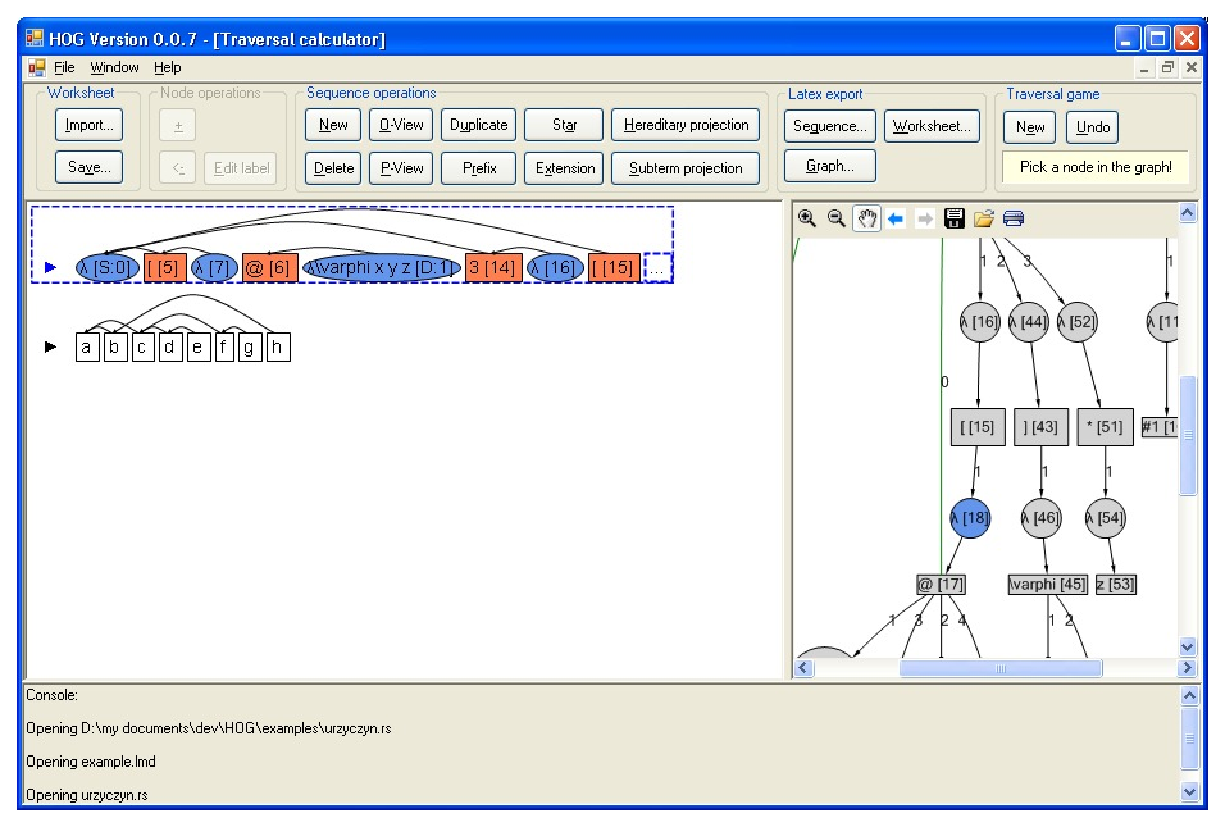
\includegraphics[width=15cm]{sshot_traversal}\\
\end{bigcenter}
  \caption{Screenshot of a traversal game in \toolname.}
  \label{fig:sshot_hog_traversal}
\end{figure}

The right-hand side of the window contains a representation of the computation graph and the left part of the window contains a list of justified sequences created by the user. In the screenshot, the first justified sequence corresponds to a traversal that is being played by the user. Opponent moves and Proponent moves are represented by circles and rectangular nodes respectively. The user make a move by selecting a node among the valid nodes highlighted in the computation graph. If there is a unique possible
 justifier in the traversal then the move is automatically
accepted, otherwise the user has to specify a move by selecting a valid justifier in the traversal. After the move is accepted \toolname\ responds with a P-move. This goes on until the traversal is maximal.

\toolname\ allows the user to perform several operations on the justified sequence such as computing the P-view or the O-view. It is also possible to export the sequence to \LaTeX\ code. For example, typesetting the traversal from Figure \ref{fig:sshot_hog_traversal} with \LaTeX\ produces
$$\Pstr[0.7cm]{(n0){\lambda }\ (n1-n0){[}\ (n2-n1){\lambda }\ (n3){@}\ (n4-n3){\lambda \varphi x y z}\ (n5-n0){3}\ (n6-n5){\lambda }\ (n7-n0){[}\ {...}\ }$$

\subsection{Other features}




\subsubsection{Generating a CPDA from a recursion scheme}
\toolname\ can  convert any higher-order recursion scheme into an equivalent (\ie generating the same infinite tree) Collapsible Push-down Automaton (CPDA) of the same order. The algorithm used to perform this transformation is taken from \cite{hague-sto07}.

The transition function of a CPDA is given by a list of instructions which we call the ``code'' of the CPDA. Figure \ref{fig:cpda_listing} give an example of CPDA generated from the Urzyczin recursion scheme.

\begin{figure}
\begin{lstlisting}[breaklines=true,basicstyle=\tiny]
Order: 2

Stack alphabet: 0 1 2 3 4 5 6 7 8 9 10 11 12 13 14 15 16 17 18 19 20 21 22 23 24 25 26 27 28 29 30 31 32 33 34 35 36 37 38 39 40 41 42 43 44 45 46 47 48 49 50 51 52 53 54 55 56 57 58 59

Code:
Code:

    0                   PUSH1 0 (0,0)
    1 start          :  CASETOP0 0->NODE0 1->NODE1 2->NODE2 3->NODE3 4->NODE4 5->NODE5 6->NODE6 7->NODE7 8->NODE8 9->NODE9 10->NODE10 11->NODE11 12->NODE12 13->NODE13 14->NODE14 15->NODE15 16->NODE16 17->NODE17 18->NODE18 19->NODE19 20->NODE20 21->NODE21 22->NODE22 23->NODE23 24->NODE24 25->NODE25 26->NODE26 27->NODE27 28->NODE28 29->NODE29 30->NODE30 31->NODE31 32->NODE32 33->NODE33 34->NODE34 35->NODE35 36->NODE36 37->NODE37 38->NODE38 39->NODE39 40->NODE40 41->NODE41 42->NODE42 43->NODE43 44->NODE44 45->NODE45 46->NODE46 47->NODE47 48->NODE48 49->NODE49 50->NODE50 51->NODE51 52->NODE52 53->NODE53 54->NODE54 55->NODE55 56->NODE56 57->NODE57 58->NODE58 59->NODE59
    2 NODE0          :  PUSH1 5 (1,1)
    3                   GOTO start
    4 NODE1          :  PUSH1 14 (1,1)
    5                   GOTO start
    6 NODE2          :  PUSH1 55 (1,1)
    7                   GOTO start
    8 NODE3          :  PUSH1 58 (1,1)
    9                   GOTO start
   10 NODE4          :  PUSH1 59 (1,1)
   11                   GOTO start
   12 NODE5          :  EMIT [ NODE5_1
   13 NODE5_1        :  PUSH1 7 (0,0)
   14                   GOTO start
   15 NODE6          :  PUSH1 1 (1,1)
   16                   GOTO start
   17 NODE7          :  PUSH1 6 (1,1)
   18                   GOTO start
   19 NODE8          :  PUSH1 4 (1,1)
   20                   GOTO start
   21 NODE9          :  PUSH1 8 (1,1)
   22                   GOTO start
   23 NODE10         :  REPEAT 3 TIMES POP1
   24                   COLLAPSE
   25                   CASETOP0 45->NODE10_45 21->NODE10_21
   26                   FAILWITH "Unexpected top 0-element!"
   27 NODE10_21      :  PUSH1 24 (3,1)
   28                   GOTO start
  ...
\end{lstlisting}
\label{fig:cpda_listing}
\caption{Excerpt of the listing of the CPDA generated  from the Urzyczin recursion scheme.}
\end{figure}

A line of code of the CPDA is made of three parts: the line number, an optional label and an instruction. There are four kinds of instructions: stack instructions, the node emitting instruction, branching instructions and debugging instructions. The stack instructions are:
\begin{description}
  \item[{\tt PUSH1 a (j,k)}] push the element {\tt a} on the top 1-stack an associates the link $(j,k)$ to it. This encoding means that the link points to a prefix stack obtained by performing an order-$j$ pop $k$ consecutive times.
  \item[{\tt PUSHn}] performs an order $n$ push on the stack (duplicates the top $n-1$-stack).
  \item[{\tt POPn}] performs an order $n$ pop on the stack (pop the top $n-1$-stack).
  \item[{\tt COLLAPSE}] collapses the stack to the prefix stack pointed to by the top element in the stack. In other words it executes $k$ times the execution {\tt POPj} where {\tt (j,k)} is the encoding of the link associated to the top element.

  \item[{\tt REPEAT n TIMES ins}] repeats the instruction {\tt ins} $n$ times where $n$ is a constant. The behaviour is unspecified if {\tt ins} is a branching instruction.
\end{description}

In order to create nodes in the value-tree, the CPDA uses teh following special instruction:
\begin{description}
  \item[$\mathtt{EMIT\ f\ LAB_1 \ldots LAB_k}$] emits the terminal $f$ of type $o^k \rightarrow o$.
   The CPDA is then spawn into $k$ other CPDA's, one for each parameter of the terminal $f$.
   The $i's$ spawn CPDA will be started at instruction $\mathtt{LAB_i}$ for $i \in \{1..k\}$.
\end{description}

The branching instructions are:
\begin{description}
  \item[{\tt GOTO lab}] jumps to the label {\tt lab}.
  \item[$\mathtt{CASTOP0\ e_0->lab_0 ... e_k->lab_k}$] performs a test case on the element
  at the top of the stack. If the top element is equal to $\mathtt{e_i}$ for some $i \in \{0..k\}$
  then the CPDA jumps to the label $\mathtt{lab_k}$. Otherwise it moves on to the following instruction.
\end{description}

There are also instructions used for debugging the code of a CPDA:
\begin{description}
  \item[{\tt FAILWITH msg}] raises an exception with the message {\tt msg}.
  \item[{\tt ASSERT msg}] asserts that the condition described by the message {\tt msg} is verified. If the test fails then an exception is raised.
\end{description}



A configuration of the CPDA is given by an instruction number together with an order-$n$ stack. In the initial configuration, the CPDA is positioned on the first instruction and the stack is the empty order-$n$ stack. After executing a transition the CPDA moves to the next instruction (or jump to another line if it is a branching instruction).




\subsubsection{Exploring the value tree by executing the CPDA transitions }

When you open a CPDA, \toolname\ displays a lazy value tree (Figure \ref{fig:sshot_cpda}). Each node of this tree corresponds to a configuration of the CPDA. Nodes are either labelled by an instruction number or by a terminal. In a separate textbox, \toolname\ shows the content of the stack for the selected configuration.

\begin{figure}
\begin{bigcenter}
  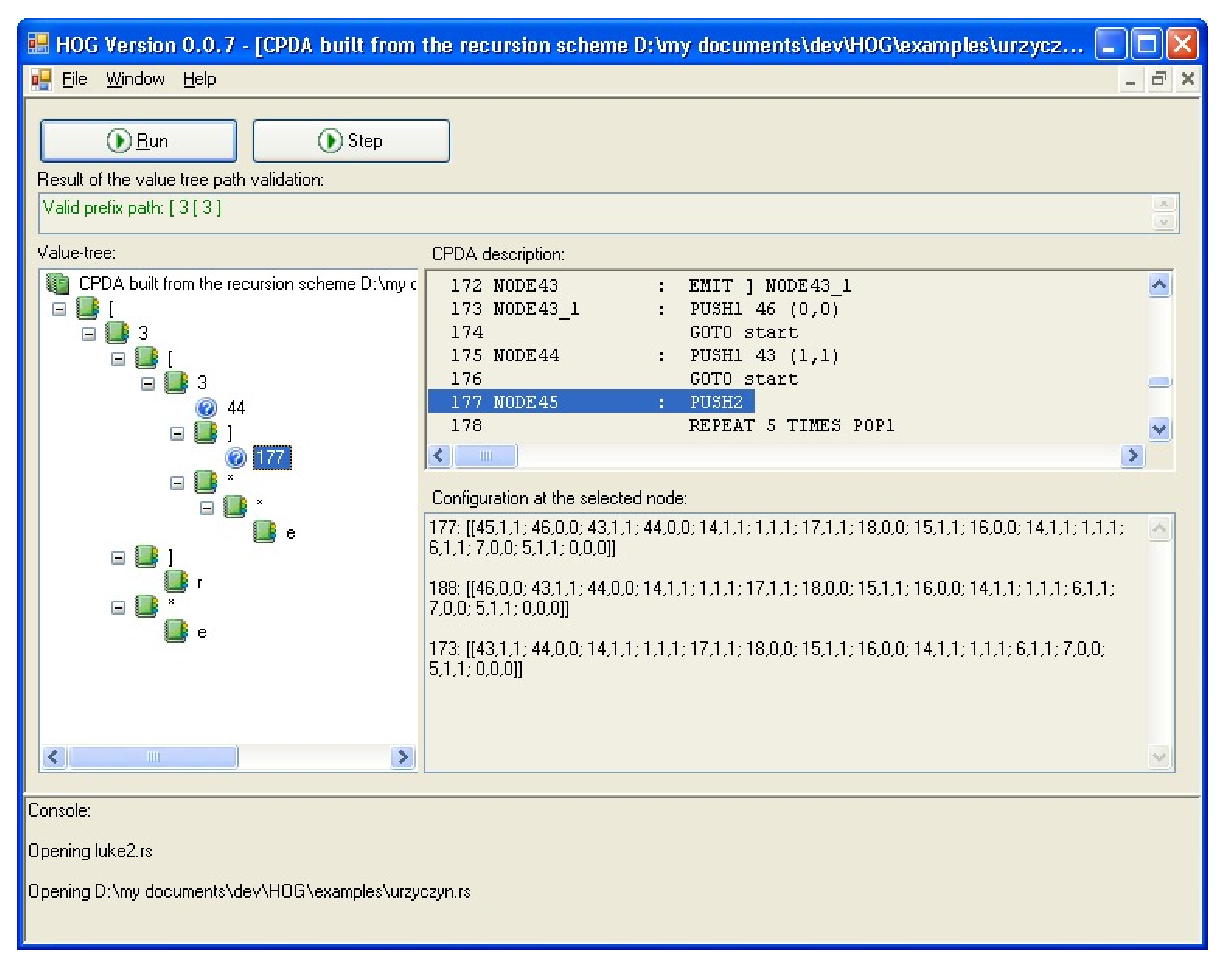
\includegraphics[width=14cm]{sshot_cpda}\\
\end{bigcenter}
  \caption{\toolname\ executing the CPDA generated from the Urzyczin recursion scheme.}
  \label{fig:sshot_cpda}
\end{figure}

Initially, the root node is labeled with the instruction number $0$ which corresponds to the first instruction of the CPDA code. When executing the CPDA transition on a node, the stack is updated accordingly and the node label is updated to the next instruction to be executed. This process is repeated until reaching an {\tt EMIT} instruction.

When an instruction $\mathtt{EMIT\ f\ LAB_1 \ldots LAB_k}$ is executed (which means that a terminal $f:o^k\rightarrow o$ is emitted), a node labelled $f$ is created in the value tree with $k$ children nodes are attached to it. Each child corresponds to a newly spawn CPDA with the same stack as in the original configuration. Finally, the current instruction of the  $i$th child is set to the instruction number with label $\mathtt{LAB_i}$.

Terminal nodes represent the actual nodes of the value-tree and as such cannot be expanded further.

\subsubsection{Exploring the tree generated by a recursion scheme}

\toolname\ has another feature which allows one to explore the infinite tree generated from a given recursion scheme without the need to convert it into a CPDA beforehand.


    \bibliographystyle{plain}
    \bibliography{../bib/dphil-all}

\end{document}

\usepackage{graphicx}
\usepackage{url}
\def\toolname{HOG}


\title{A tool illustrating the Correspondence Theorem
\\ GALOP 2008}

\author{William~Blum~~~~~~~~~~~C.-H.~Luke~Ong\\
Oxford University Computing Laboratory\\
Wolfson Building, Parks Road, Oxford OX1 3QD, ENGLAND\\
\{william.blum,luke.ong\}@comlab.ox.ac.uk }



\begin{document}
\maketitle \thispagestyle{empty}

\begin{abstract}
Todo...
\end{abstract}

\tableofcontents

\section{Luke's description of the paper:}

 We have developed a number of what we call Path-Traversal
Correspondence Theorems. One way to think of the work is as a kind of representation theory of the game semantics of higher-type programs (such as recursion schemes, PCF and Idealized Algol) that is very concrete, involving combinatorics over (possibly) infinite structures defined by the abstract syntax trees of the programs being modelled. The idea is that we represent a play in the strategy-denotation of a term as the underlying "hereditarily uncovered" interaction sequence, called traversal. Another way to put it is that traversals are built up by performing parallel-composition but WITHOUT the hiding. This is what William Greenland has called (in his thesis) "revealed semantics" (or "interaction semantics"). A consequence of the representation is that we show how the "innocent game" given by a term can be played out very concretely over what is in essence the abstract syntax tree of the term itself.

This "representation theory" was first developed to prove the result in my LICS06 paper (i.e. trees generated by higher-order recursion schemes have decidable MSO theories). The theory has at least two other applications. First as a justification of the game characterization of the Higher-Order Matching Problem (but NOT the algorithm) developed by Colin Stirling, and secondly as a key lemma underpinning the result that
 the following are equivalent (i.e. equi-expressive:
i. order-n recursion schemes (= order-n PCF terms generated from uninterpreted order-1 symbols) ii. order-n collapsible pushdown automata CPDA. iii. order-n "pure" innocent strategies

What we are thinking of submitting is a short paper describing a tool developed by William Blum that illustrates the representation theory. The tool has many capabilities. For example, it can perform the inter-translation between CPDA and recursion schemes; it can demonstrate the path-traversal correspondence in the form of a 2-player game (and lets users play it out over the abstract syntax tree of the term); and it is a very impressive tool for drawing justified sequences!

What we intend to talk about in the paper is first an overview of the correspondence theorems, illustrate their many applications, and then showcase the tool.

\section{Computation tree, Traversals and the Correspondence Theorem}

In \cite{OngLics2006}, one of us introduced the notion of computation tree and traversals over a computation tree for the purpose of studying trees generated by higher-order recursion scheme. Here we extend these concepts to the pure (\ie without constants) simply-typed lambda calculus. Our setting allows the presence of free variable of any order. Moreover the term studied is not necessarily of ground type. (This contrasts with \cite{OngLics2006}'s setting where the term is of ground type and contains only \emph{uninterpreted constant}\footnote{A constant $f$ is  \emph{uninterpreted} if the small-step semantics of the language
  does not contain any rule of the form $f \dots \rightarrow e$. $f$
  can be regarded as a data constructor.} of order 1 at most and no
free variables.) Note that our setting automatically accounts for the presence of uninterpreted constants since they can be regarded as free variables. We will then state the \emph{Correspondence Theorem} (Theorem \ref{thm:correspondence}).

In the following we fix a simply-typed term $\Gamma \vdash M :T$.

\subsection{Computation tree}
 In \cite{OngLics2006} the computation tree of a grammar is
defined as the unravelling of a finite graph representing the long transform of a grammar. Similarly we define the computation tree of a $\lambda$-term as an abstract syntax tree of its $\eta$-long normal form.  We write $l\langle t_1, \ldots, t_n \rangle$ with $n \geq 0$ to denote the tree with a root labelled $l$ with $n$ children subtrees $t_1$, \ldots, $t_n$.

\begin{definition}\rm
\label{dfn:comptree}
  The \defname{computation tree} $\tau(M)$ of a simply-typed term
  $\Gamma \vdash M:T$ with variable names in a countable set
  $\mathcal{V}$ is a tree with labels in $ \{ @ \} \union \mathcal{V}
  \union \{ \lambda x_1 \ldots x_n \ | \ x_1 ,\ldots, x_n \in
  \mathcal{V}, n\in\nat \}$ defined from its $\eta$-long form as follows.
  Let $\overline{x}$ denote some list of variables $x_1 \ldots x_n$ for some $n\geq 0$.
\begin{eqnarray*}
  \mbox{For $m\geq 0$, $z \in \mathcal{V}$: } \tau(\lambda \overline{x} . z s_1 \ldots s_m ) &=& \lambda \overline{x} \langle z \langle\tau(s_1),\ldots,\tau(s_m)\rangle\rangle \\
  \mbox{For $m \geq 1$: } \tau(\lambda \overline{x} . (\lambda y.t) s_1 \ldots s_m) &=& \lambda \overline{x} \langle @ \langle \tau(\lambda y.t),\tau(s_1),\ldots,\tau(s_m) \rangle \rangle \ .
\end{eqnarray*}
\end{definition}

Even-level nodes are $\lambda$-nodes (the root is on level 0). A single $\lambda$-node can represent several consecutive variable abstractions or it can just be a \emph{dummy lambda} if the corresponding subterm is of ground type.  Odd-level nodes are variable or application nodes.

We say that a variable node $n$ labelled $x$ is \defname{bound} by a node $m$, and $m$ is called the \defname{binder} of $n$, if $m$ is the closest node in the path from $n$ to the root such that $m$ is labelled $\lambda \overline{\xi}$ with $x\in \overline{\xi}$.


We write $\theroot$ to denote the root of the computation tree $\tau(M)$. The set of nodes of the computation tree is denoted by $N$. The sets $N_@$, $N_\lambda$ and $N_{\sf var}$ are the subset of $N$ consisting of the @-nodes, $\lambda$-nodes and variable nodes respectively.


\subsection{Justified sequences of nodes}

We define the \defname{enabling relation} on the set of nodes of the computation tree as follows: $m$ enables $n$, written $m \vdash n$, if and only if $n$ is bound by $m$ (and we sometimes write $m \vdash_i n$ to precise that $n$ is the $i^{\sf th}$ variable bound by $m$); or $m$ is the root $\theroot$ and $n$ is a free variable; or $n$ is a $\lambda$-node and $m$ is its parent node.


We say that a node $n_0$ of the computation tree is
\defname{hereditarily enabled} by $n_p \in N$ if there are nodes
$n_1,\ldots, n_{p-1} \in N$ such that $n_{i+1}$ enables $n_{i}$ for all $i\in 0..p-1$.

For any set of nodes $S, H \subseteq N$ we write $S^{H\vdash}$ for $S \inter \vdash^*(H) = \{ n \in S \ | \exists n_0 \in H \mbox{ s.t. }n_0  \vdash^* n \}$ -- the subset of $S$ constituted of nodes hereditarily enabled by some node in $H$. We will abbreviate $S^{\{n_0\}\vdash}$ into $S^{n_0\vdash}$.

We call \defname{input-variables nodes} the elements of $V_{\sf var}^{\theroot\vdash}$ \ie variables that are hereditarily enabled by the root of $\tau(M)$. Thus we have $V_{\sf var}^{\theroot\vdash} = V \setminus ( V_{\sf var}^{N_@\vdash} \union V_{\sf var}^{N_\Sigma\vdash})$.

A \defname{justified sequence of nodes} is a sequence of nodes with pointers such that each occurrence of a variable or $\lambda$-node $n$ different from the root has a pointer to some preceding occurrence $m$ verifying $m \vdash n$. In particular, occurrences of @-nodes do not have pointer. We represent the pointer in the sequence as follows \Pstr[0.4cm]{ (m){m} \ldots (n-m,45:i) n }.
 where the label indicates that either $n$ is labelled with the $i$th variable
abstracted by the $\lambda$-node $m$ or that $n$ is the $i^{\sf th}$ child of $m$.  Children nodes are numbered from $1$ onward except for @-nodes where it starts from $0$. Abstracted variables are numbered from $1$ onward. The $i^{\sf th}$ child of $n$ is denoted by $n.i$.

We say that a node $n_0$ of a justified sequence is
\defname{hereditarily justified} by $n_p$ if there are occurrences $n_1,
\ldots, n_{p-1}$ in the sequence such that $n_i$ points to $n_{i+1}$ for all $i\in 0..p-1$. Let $n$ be an occurrence in a justified sequence $s$. We write $s \filter r$ to denote the subsequence of $s$ consisting of the occurrences hereditarily justified by $n$.


The notion of \defname{P-view} $\pview{t}$ of a justified sequence of nodes $t$ is defined the same way as the P-view of a justified sequences of moves in Game Semantics:\footnote{ The equalities in the
  definition determine pointers implicitly. For instance in the second
  clause, if in the left-hand side, $n$ points to some node in $s$
  that is also present in $\pview{s}$ then in the right-hand side, $n$
  points to that occurrence of the node in $\pview{s}$.}
$$\begin{array}{rclrcl}
\pview{\epsilon} &=&  \epsilon & \pview{\Pstr[0.5cm]{ s \cdot (m) m \cdot \ldots \cdot (lmd-m,40){\lambda\overline{\xi}} }}
 &=& \Pstr{
\pview{s} \cdot (m2) m \cdot (lm2-m2,50) {\lambda \overline{\xi}} } \\
\mbox{for $n \notin N_\lambda$, } \pview{s \cdot n }  &=&  \pview{s} \cdot n \qquad & \pview{s \cdot \theroot }  &=&  \theroot
\end{array}$$

The O-view of $s$, written $\oview{s}$, is defined dually. We will borrow the game semantic terminology: A justified sequences of nodes satisfies \defname{alternation} if for any two consecutive nodes one is a $\lambda$-node and the other is not, and \defname{P-visibility} if every variable node points to a node occurring in the P-view a that point.

\subsection{Adding value-leaves to the computation tree}

We now add another ingredient to the computation tree that was not originally used in \cite{OngLics2006}.  We write $\mathcal{D}$ to denote the set of values of the base type $o$.  We add
\defname{value-leaves} to $\tau(M)$ as follows: For each value $v
\in \mathcal{D}$ and for each node $n \in N$ we attach the child leaf $v_n$ to $n$.  We write $V$ for the set of vertices of the resulting tree (\ie inner nodes and leaf nodes). For $\$$ ranging in $\{@, \lambda, var \}$, we write $V_\$$ to denote the set of inner nodes from $N_\$$ plus the leaf-nodes whose parent is in $N_\$$ \ie $V_\$ = N_\$ \union \{ v_n \ | \ n \in N_\$, v \in \mathcal{D} \}$.


Everything that we have defined can be lifted to this new version of computation tree. The enabling relation $\vdash$ is extended so that every leaf is enabled by its parent node. A link going from a value-leaf $v_n$ to a node $n$ is labelled by $v$: \Pstr[0.4cm]{ (n) n \ldots (vn-n,35:v){v_n} }. For the definition of P-view and visibility, value-leaves are treated as $\lambda$-nodes if they are at an odd level in the computation tree, and as variable nodes if they are at an even level.

We say that an occurrence of an inner node $n \in N$ is
\defname{answered} by an occurrence $v_n$ if $v_n$ in
the sequence that points to $n$, otherwise we say that $n$ is
\defname{unanswered}. The last unanswered node is called the
\defname{pending node}.  A justified sequence of nodes is
\defname{well-bracketed} if each value-leaf occurring in it is justified by the pending node at that point.  If $t$ is a traversal then we write
$?(t)$ to denote the subsequence of $t$ consisting only of unanswered nodes.

\subsection{Traversals of the computation tree}
\label{subsec:traversal}

A \emph{traversal} is a justified sequence of nodes of the computation tree where each node indicates a step that is taken during the evaluation of the term.

\begin{definition}[Traversals for simply-typed $\lambda$-terms] \rm
\label{def:traversal} The set $\travset(M)$ of \defname{traversals}
over $\tau(M)$ is defined by induction over the rules of Table
\ref{tab:trav_rules}. A traversal that cannot be extended by any
rule is said to be \emph{maximal}.
\end{definition}

\begin{FramedTable}
\noindent {\bf Initialization rules}
\begin{itemize}[]
\item\rulenamet{Empty} $\epsilon \in \travset(M)$.
\item\rulenamet{Root} The sequence constituted of a single occurrence of $\tau(M)$'s root is a traversal.
\end{itemize}

\noindent {\bf Structural rules}
\begin{itemize}[]
    \item \rulenamet{Lam} If $t \cdot \lambda \overline{\xi}$ is a traversal then so is
        $t \cdot \lambda \overline{\xi} \cdot n$ where $n$
        denotes $\lambda \overline{\xi}$'s child and:
        \begin{compactitem}
            \item If $n \in N_@ \union N_\Sigma$ then it has no justifier;
            \item if  $n \in N_{\sf var}\setminus N_{\sf fv}$ then it points to the only occurrence\footnote{Prop.\ \ref{prop:pviewtrav_is_path} will show that P-views
            are paths in the tree thus $n$'s enabler occurs
            exactly once in the P-view.} of its binder in
            $\pview{t\cdot \lambda \overline{\xi}}$;
            \item if  $n \in N_{\sf fv}$ then it points
            to the only occurrence of the root $\theroot$ in
            $\pview{t \cdot \lambda \overline{\xi}}$.
        \end{compactitem}
    \item \rulenamet{App} If $t \cdot @$ is a traversal then so is \Pstr[0.4cm]{t \cdot (m) @  \cdot (n-m,40:0) n}.
\end{itemize}

\emph{\bf Input-variable rules}
\begin{itemize}[]
\item \rulenamet{InputVar} If $t$ is a traversal where $t^\omega \in N_{\sf var}^{\theroot\vdash} \union L_\lambda^{\theroot\vdash}$
and $x$ is an occurrence of a variable node in $\oview{t}$ then
so is $t \cdot n$ for any child $\lambda$-node $n$ of $x$, $n$
pointing to $x$.



\item \rulenamet{InputValue} If $t_1
\cdot x \cdot t_2$ is a traversal with pending node $x \in
N_{\sf var}^{\theroot\vdash}$ then so is \Pstr[0.5cm]{t_1 \cdot
(x){x} \cdot t_2 \cdot (xv-x,38:v){v_x} } for all $v \in
\mathcal{D}$.
\end{itemize}

\emph{\bf Copy-cat rules}
\begin{itemize}[]
\item\rulenamet{Var}
If \Pstr[0.5cm]{t \cdot (n){n} \cdot (lx){\lambda \overline{x}}
    \ldots (x-lx,50:i){x_i} } is a traversal where $x_i \in
    N_{\sf var}^{@\vdash}$ then so is \Pstr[0.5cm]{ t \cdot
(n){n} \cdot (lx){\lambda \overline{x}}  \ldots (x-lx,30:i){x_i}
    \cdot (letai-n,40:i){\lambda \overline{\eta_i}}
     }.

\item\rulenamet{Value}
  If \Pstr{t \cdot (m){m} \cdot (n){n}  \ldots
(vn-n,60:v){v}_{n} } is a traversal where $n\in N$ then so is
\Pstr[0.6cm]{t \cdot (m){m} \cdot (n){n} \ldots
(vn-n,60:v){v}_{n} \cdot (vm-m,45:v){v}_m}.
\end{itemize}
\caption[Traversal rules for the simply-typed
lambda-calculus]{Traversal rules for the simply-typed
$\lambda$-calculus.}
 \label{tab:trav_rules}
\end{FramedTable}


\parpic[r]{
 $\pssetcomptree\tree[levelsep=3ex,treesep=0.5cm]{\lambda} {
    \tree{@}{
        \pstree[linestyle=dotted]{\TR{\lambda y}\arclabel{0} }{
            \tree{y}{
                \tree{\lambda \overline{\eta_1}}{\vdots}%\arclabel{1}
                \tree{\lambda \overline{\eta_i}}{\vdots}%\arclabel{i}
                \tree{\lambda \overline{\eta_n}}{\vdots}%\arclabel{n}
            }
        }
        \pstree[linestyle=dotted]{\TR{\lambda \overline{x}}
            \arclabel{1}}{ \tree{x_i}{\TR{} \TR{}}}
}}$ } A traversal always starts by visiting the root. Then it mainly follows the structure of the tree. The (Var) rule permits to jump across the computation tree. The idea is that after visiting a variable node $x$, a jump is allowed to the node corresponding to the subterm that would be substituted for $x$ if all the $\beta$-redexes occurring in the term were reduced. The sequence \Pstr[0.8cm]{\lambda \cdot (app) @  \cdot (ly) {\lambda y}  \ldots (y-ly,35:1) y  \cdot (lx-app,38:1) {\lambda \overline{x}} \ldots (x-lx,30:i) {x_i} \cdot (leta-y,40:i) {\lambda \overline{\eta_i} } \ldots}
 is an example of traversal of the computation tree shown on the right.

\begin{proposition}[counterpart of proposition 6 from \cite{OngHoMchecking2006}]
\label{prop:pviewtrav_is_path} Let $t$ be a traversal. Then:
\begin{enumerate}[(i)]
\item $t$ is a well-defined and well-bracketed justified sequence;
\item $t$ is a well-defined justified sequence verifying alternation, P-visibility and O-visibility;
\item If $t$'s last node is not a value-leaf, then $\pview{t}$ is the path in the computation tree going from the root to $t$'s last node.
\end{enumerate}
\end{proposition}

The \defname{reduction} of a traversal $t$ is the subsequence of $t$ obtained by keeping only occurrences of nodes that are hereditarily enabled by the root $\theroot$. This has the effect of eliminating the ``internal nodes'' of the computation. If $t$ is a non-empty traversal then the root $\theroot$ occurs exactly once in $t$ and the reduction of $t$ is equal to $t \filter r$. We write $\travset(M)^{\filter \theroot}$ for the set or reduction of traversals of $M$.

Application nodes are used to connect the operator and the operand of an application in the computation tree but since they do not play any role in the computation of the term, we can remove them from the traversals.  We write $t-@$ for the sequence of nodes-with-pointers obtained by removing from $t$ all @-nodes and value-leaves of @-nodes, any link pointing to an @-node being replaced by a link pointing to the immediate predecessor of @ in $t$. We write $\travset(M)^{-@}$ for the set $\{ t - @ \ | \  t \in \travset(M) \}$.
\begin{remark}
If $M$ is $\beta$-normal then $\tau$ does not contain any @-node therefore all nodes are hereditarily justified by $r$ and we have $\travset(M)^{-@} = \travset(M) = \travset(M)^{\filter \theroot }$.
\end{remark}

\subsection{Revealed Game Semantics}

In game semantics, strategy composition is achieved by performing a CSP-like ``composition + hiding''. If the internal moves are not hidden then we obtain an alternative semantics called \emph{revealed semantics} in \cite{willgreenlandthesis} and \emph{interaction} semantics in \cite{DBLP:conf/sas/DimovskiGL05}. Here we will refer to this semantics as the \defname{fully revealed game semantics}. The fully revealed game denotation of a term $\Gamma \vdash M :T$, written $\revsem{\Gamma \vdash M : T}$, is obtained by uncovering\footnote{An algorithm that uniquely recovers hidden moves is given in Part II of
  \cite{hylandong_pcf}.} all the internal moves from $\sem{\Gamma \vdash
  M : T}$ generated during strategy composition.
We introduce a variation of the fully-revealed game denotation called the \defname{syntactically-revealed game denotation}, written $\syntrevsem{\Gamma \vdash
  M : T}$. In this denotation, as opposed to the fully-revealed denotation,
only \emph{certain} internal moves from $\sem{\Gamma \vdash
  M : T}$ are uncovered: The internal moves that are generated by the composition with the evaluation map
$ev$ at a @-node of the computation tree are all uncovered, but in the denotation of a subtem of the form $y N_1 \ldots N_p$ for some $p\geq1$, only certain internal moves are uncovered. The formal definition can be found in \cite{localbeta2008}.

\subsection{Computation trees and arenas}
We consider the well-bracketed game model of the simply-typed lambda calculus.  We choose to represent strategies using ``prefix-closed set of plays''. \footnote{In the literature, a strategy is usually defined as a set of plays closed by \emph{even}-length prefix. For the purpose of showing the Correspondence Theorem, however, the ``prefix-closed''-based definition is more adequate.} We fix a term $\Gamma \vdash M : T$ and write $\sem{\Gamma \vdash M : T}$ for its strategy denotation. The answer moves of a question $q$ are written $v_q$ where $v$ ranges in $\mathcal{D}$.

\begin{proposition}
There exists a function $\varphi_M$, constructible from $\tau(M)$, that maps nodes from $V\setminus (V_@ \union V_\Sigma)$ to moves of the interaction arena underlying the revealed strategy $\syntrevsem{\Gamma \vdash M : T}$ and such that $\varphi$ maps $\lambda$-nodes to O-questions, variable nodes to P-questions, value-leaves of $\lambda$-nodes to P-answers and value-leaves of variable nodes to O-answers.
\end{proposition}

\begin{example}
Take $\lambda x . (\lambda g . g x) (\lambda y . y)$ with $x,y:o$ and $g:(o,o)$. The diagram below represents the computation tree (middle), the arenas $\sem{(o,o), o}$ (left), $\sem{o , o}$ (right), $\sem{o\rightarrow o}$ (rightmost) and $\varphi = \psi \union \psi_{\lambda g.g x}^{\lambda g, q_{\lambda g}} \union \psi_{\lambda y.y}^{\lambda y, q_{\lambda y}}$ (dashed-lines).
$$\psset{levelsep=3.5ex}
\pstree{\TR[name=root]{\lambda x}} {
    \pstree{\TR[name=App]{@}}
    {
            \pstree{\TR[name=lg]{\lambda g}}
                { \pstree{\TR[name=lgg]{g}}{
                        \pstree{\TR[name=lgg1]{\lambda}}
                        { \TR[name=lgg1x]{x}  } } }
            \pstree{\TR[name=ly]{\lambda y}}
                    {\TR[name=lyy]{y}}
    }
} \rput(4.5cm,-1cm){
  \pstree{\TR[name=A1lx]{q_{\lambda x}}}
        { \TR[name=A1x]{q_x} }
} \rput(-6cm,-1.5cm){
    \pstree{\TR[name=A2lg]{q_{\lambda g}}}
    {
        \pstree{\TR[name=A2g]{q_g}}
        {  \TR[name=A2g1]{q_{g_1}}   }
    }}
\rput(2.5cm,-1.5cm){
    \pstree{\TR[name=A3ly]{q_{\lambda y}}}
        { \TR[name=A3y]{q_y}
        }
} \psset{nodesep=1pt,arrows=->,arcangle=-20,arrowsize=2pt 1,linestyle=dashed,linewidth=0.3pt} \ncline{->}{root}{A1lx} \mput*{\psi} \ncarc{->}{lgg1x}{A1x} \ncline{->}{lg}{A2lg} \mput*{\psi_{\lambda g.g x}^{\lambda g, q_{\lambda g}}} \ncline{->}{lgg}{A2g} \ncline{->}{lgg1}{A2g1} \ncline{->}{ly}{A3ly} \mput*{\psi_{\lambda y.y}^{\lambda y, q_{\lambda y}}} \ncline{->}{lyy}{A3y}
$$
\end{example}

We extend the function $\varphi$ to justified sequences of nodes as follows: If $t = t_0 t_1 \ldots$ is a justified sequence of nodes in $V_\lambda \union V_{\sf var}$ then $\varphi(t)$ is defined to be the sequence of moves $\varphi(t_0)\ \varphi(t_1) \ldots$ equipped with the pointers of $t$.


\subsection{The Correspondence Theorem}


In the simply-typed lambda calculus, the set $\travset(M)$ of traversals of the computation tree is isomorphic to the set of plays of the syntactically-revealed denotation. Moreover the set of traversal reductions is isomorphic to the standard strategy denotation:

\begin{theorem}[The Correspondence Theorem]
\label{thm:correspondence} The function $\varphi_M$ gives us the following two isomorphisms:
\begin{eqnarray*}
(i)~\varphi_M  &: \travset(M)^{-@} \stackrel{\cong}{\longrightarrow} \syntrevsem{\Gamma \vdash M :T} \\
(ii)~\varphi_M  &: \travset(M )^{\filter \theroot} \stackrel{\cong}{\longrightarrow} \sem{\Gamma \vdash M : T} \ .
\end{eqnarray*}
\end{theorem}

\begin{example}
Take $M = \lambda f z . (\lambda g x . f x) (\lambda y. y) (f z) : ((o,o),o, o)$.  The figure below represents the computation tree (left tree), the arena $\sem{((o,o),o, o)}$ (right tree) and $\psi_M$ (dashed line). (Only question moves are shown for clarity.) The justified sequence of nodes $t$ defined hereunder is an example of traversal:

\begin{tabular*}{\textwidth}{lcp{6.3cm}}
$\pssetcomptree\pstree[levelsep=2.5ex,treesep=0.3cm]{ \TR[name=root]{\lambda f z} }
     {  \tree[levelsep=4ex]{@}
        {   \tree{\lambda g x}{
                  \pstree{\TR[name=f]{f^{[1]}}}{
                            \pstree{\TR[name=lmd]{\lambda^{[2]}}}
                                {\TR{x}}
                  }
                }
            \tree{\lambda y }{\TR{y}}
            \tree{\lambda ^{[3]}}{
                \pstree{\TR[name=f2]{f^{[4]}}} {
                \pstree{\TR[name=lmd2]{\lambda^{[5]}}}{\TR[name=z]{z}}
                }
            }
        }
     }
\hspace{1cm}
  \pstree[levelsep=8ex, treesep=0.3cm]{ \TR[name=q0]{q^0} }
    {   \pstree[levelsep=4ex]{\TR[name=q1]{q^1}} {\TR[name=q2]{q^2}}
        \TR[name=q3]{q^3}
    }
\psset{nodesep=1pt,arrows=->,arrowsize=2pt 1,linestyle=dashed,linewidth=0.3pt} \ncline{->}{root}{q0} \mput*{\psi_M} \ncarc[arcangle=-25]{->}{z}{q3} \ncarc[arcangle=10]{->}{f}{q1} \ncarc[arcangle=10]{->}{lmd}{q2} \ncline{->}{f2}{q1} \ncline{->}{lmd2}{q2}$ &  &
\begin{asparablank}
  \item  \Pstr[0.8cm]{
t = (n){\lambda f z} \ (n2){@} \ (n3-n2,60){\lambda g x} \ (n4-n,45){f^{[1]}} \ (n5-n4,45){\lambda^{[2]}} \ (n6-n3,45){x} \ (n7-n2,35){\lambda^{[3]}} \ (n8-n,35){f^{[4]}} \ (n9-n8,45){\lambda^{[5]}} \ (n10-n,35){z} }

\item \Pstr[0.9cm]{
t\filter r = (n){\lambda f z} \ (n4-n,50){f}^{[1]} \ (n5-n4,60){\lambda}^{[2]} \ (n8-n,45){f}^{[4]} \ (n9-n8,60){\lambda}^{[5]} \ (n10-n,40){z}}
\item
\Pstr[0.8cm]{ {\varphi_M(t\filter r) =\ } (n){q^0}\ (n4-n,60){q^1}\ (n5-n4,60){q^2}\ (n8-n,45){q^1}\ (n9-n8,60){q^2}\ (n10-n,38){q^3} \in \sem{M}\ .}
\end{asparablank}
\end{tabular*}
\end{example}


\section{Presentation of the tool}

We have developed a tool called \toolname\ that permits one to visualize and explore the Traversal-Game Semantics Correspondence presented in the previous section. The binary files and sources in OCaml/F\# can be downloaded from \url{http://web.comlab.ox. ac.uk/oucl/work/william.blum/}.

\subsection{Generation of the computation graph/tree}

\toolname\ accepts two kind of objects as an input: simply-typed terms or higher-order recursion schemes. A recursion scheme is a special kind of higher-order grammar that can be used to generated an infinite tree called the value-tree (not to be confused with the computation tree). A recursion scheme can be thought as a simply-typed term of ground type extended with recursion and containing uninterpreted constant of order at most 1 (used to represent the constructors for the nodes of the value tree). Since recursion schemes allow the use of recursion, the computation tree becomes a computation \emph{graph}. Traversal are however defined in the same way and the Correspondence Theorem still holds. This setting was originally treated in \cite{OngLics2006} where the concepts of computation tree and traversal were introduced.


\toolname\ allows you to generate the computation tree of a higher-order simply-typed term as well as the computation graph of a higher-order recursion scheme.

\subsection{Example}

Take for instance the Urzyczin recursion scheme (see \cite{demirandathesis}). It is formally given by the tuple $\langle \Sigma, \mathcal{N}, \mathcal{R}, S \rangle $ where the set of terminals is $\Sigma = \{[:o\typear o,
    ]:o \typear o,*:o \typear o, 3:o \typear o \typear o \typear o, e:o,
    r:o\}$, the set of non-terminals is
 $\mathcal{N} = \{ S:o,
    D:(o \typear o \typear o) \typear o \typear o \typear o \typear
    o,
    F:o \typear o,
    E:o,
    G:o \typear o \typear o \}$ and the set of rules $\mathcal{R}$ is given by
\[\begin{array}{rll}
   S\, & \rightarrow & [\, (D\, G\, E\, E\, E\,) \\
    D\, \varphi x y z & \rightarrow & 3 ([ (D\, (D\, \varphi\, x)\, z\, (F\, y) (F\, y))) (] (\varphi\, y\, x)) (* z) \\
    F\, x & \rightarrow & *\, x \\
    E\, & \rightarrow & e \\
    G\, u v & \rightarrow & r
\end{array}\]


Using the \toolname\ syntax this is expressed as follows:
\begin{lstlisting}[breaklines=true]
name { "Urzyczin tree" } validator { demiranda_urzyczyn } terminals{
    [:o-> o;
    ]:o -> o;
    *:o -> o;
    3:o -> o -> o -> o;
    e:o;
    r:o; }
nonterminals {
    S:o ;
    D:(o -> o -> o) -> o -> o -> o -> o ;
    F:o -> o ;
    E:o;
    G:o -> o -> o; }
rules {
    S = [ (D G E E E) ;
    D \varphi x y z = 3 ([ (D (D \varphi x) z (F y) (F y))) (] (\varphi y x)) (* z);
    F x = * x ;
    E = e ;
    G u v = r ; }
\end{lstlisting}

Figure \ref{fig:urz_graph} represents the computation graph. (The \TeX\ source code for this graph is automatically generated by \toolname.) The framed nodes correspond to the constant nodes.

\begin{figure}[htbp]
\begin{bigcenter}
\psset{levelsep=5ex,linewidth=0.5pt,nodesep=1pt,arcangle=-20,arrowsize=2pt 1} \setlength\fboxsep{2pt}
%\newcommand{\pssetcomptree}{\psset{levelsep=4ex,linewidth=0.5pt}}
\pssetcomptree $\pstree{\TR{[S]\lambda }}{\pstree{\TR{\framebox{[}}}{\pstree{\TR{\lambda }}{\pstree{\TR{@}}{\pstree{\TR[name=1]{[D]\lambda \varphi x y z}\ncput*{\scriptstyle 0}}{\pstree{\TR{\framebox{3}}}{\pstree{\TR{\lambda }}{\pstree{\TR{\framebox{[}}}{\pstree{\TR{\lambda }}{\pstree{\TR[name=n0]{@}}{\pstree{\TR{\lambda \theta_{3} \theta_{4}}}{\pstree{\TR[name=n1]{@}}{\pstree{\TR{\lambda \theta_{5} \theta_{6}}}{\pstree{\TR{\varphi}}{\pstree{\TR{\lambda }}{\TR{\theta_{5}}} \pstree{\TR{\lambda }}{\TR{\theta_{6}}}}} \pstree{\TR{\lambda }}{\TR{x}} \pstree{\TR{\lambda }}{\TR{\theta_{3}}} \pstree{\TR{\lambda }}{\TR{\theta_{4}}}}} \pstree{\TR{\lambda }}{\TR{z}} \pstree{\TR{\lambda }}{\pstree{\TR{@}}{\pstree{\TR[name=2]{[F]\lambda x}\ncput*{\scriptstyle 0}}{\pstree{\TR{\framebox{*}}}{\pstree{\TR{\lambda }}{\TR{x}}}}\pstree{\TR{\lambda }}{\TR{y}}}} \pstree{\TR{\lambda }}{\pstree{\TR[name=n2]{@}}{\pstree{\TR{\lambda }}{\TR{y}}}}}}}} \pstree{\TR{\lambda }}{\pstree{\TR{\framebox{]}}}{\pstree{\TR{\lambda }}{\pstree{\TR{\varphi}}{\pstree{\TR{\lambda }}{\TR{y}} \pstree{\TR{\lambda }}{\TR{x}}}}}} \pstree{\TR{\lambda }}{\pstree{\TR{\framebox{*}}}{\pstree{\TR{\lambda }}{\TR{z}}}}}}\pstree{\TR{\lambda \theta_{1} \theta_{2}}}{\pstree{\TR{@}}{\pstree{\TR{[G]\lambda u v}\ncput*{\scriptstyle 0}}{\TR{\framebox{r}}}\pstree{\TR{\lambda }}{\TR{\theta_{1}}} \pstree{\TR{\lambda }}{\TR{\theta_{2}}}}} \pstree{\TR[name=3]{[E]\lambda }}{\TR{\framebox{e}}} \pstree{\TR[name=3]{[E]\lambda }}{\TR{\framebox{e}}} \pstree{\TR[name=3]{[E]\lambda }}{\TR{\framebox{e}}}}}}} \ncarc{->}{n2}{2}\ncput*{\scriptstyle 0} \ncarc{->}{n1}{1}\ncput*{\scriptstyle 0} \ncarc{->}{n0}{1}\ncput*{\scriptstyle 0}$
\end{bigcenter}
  \caption{Computation graph of the Urzyczin's recursion scheme.}
  \label{fig:urz_graph}
\end{figure}


\subsection{Playing the traversal game}

Once a computation tree/graph is loaded, \toolname\ allows you to play a traversal game over it. The user plays for the Opponent while \toolname\ plays for the Proponent. Figure \ref{fig:sshot_hog_traversal} shows a screenshot of the tool when a traversal game is played.
\begin{figure}
\begin{bigcenter}
  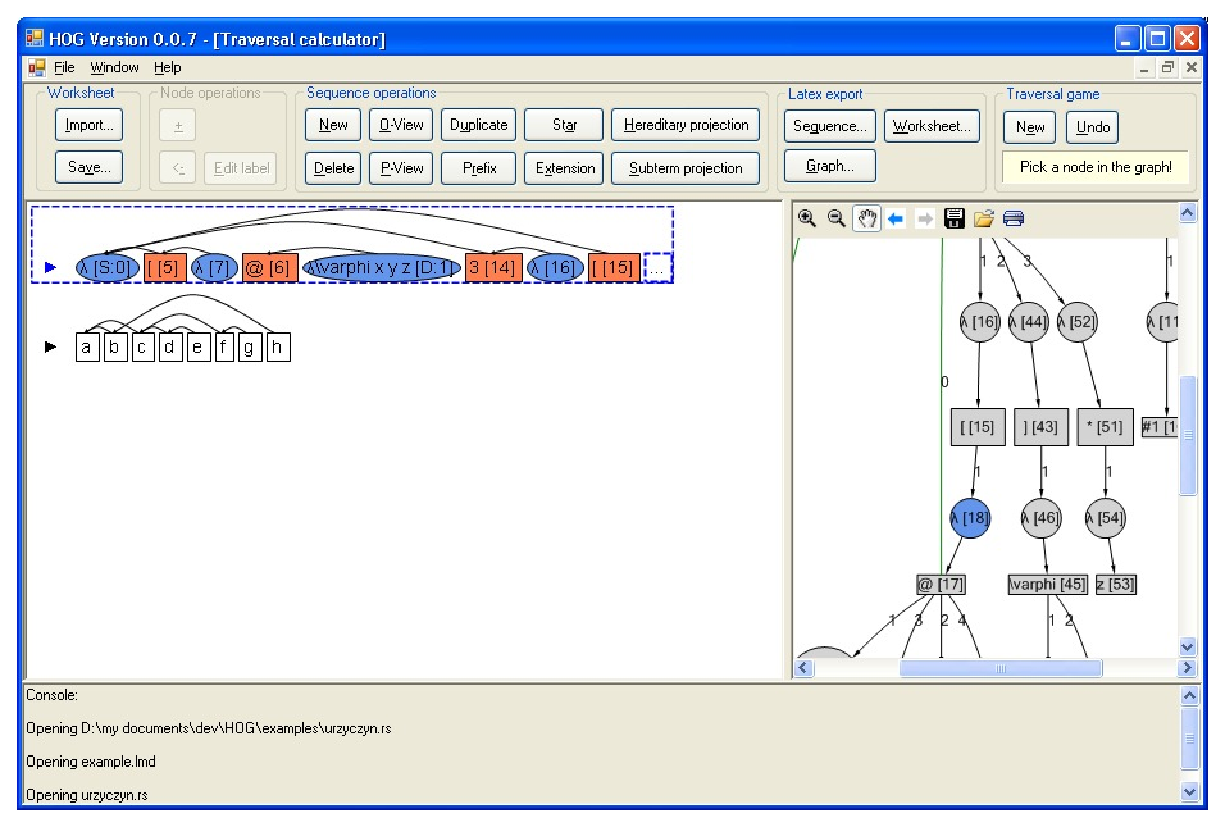
\includegraphics[width=15cm]{sshot_traversal}\\
\end{bigcenter}
  \caption{Screenshot of a traversal game in \toolname.}
  \label{fig:sshot_hog_traversal}
\end{figure}

The right-hand side of the window contains a representation of the computation graph and the left part of the window contains a list of justified sequences created by the user. In the screenshot, the first justified sequence corresponds to a traversal that is being played by the user. Opponent moves and Proponent moves are represented by circles and rectangular nodes respectively. The user make a move by selecting a node among the valid nodes highlighted in the computation graph. If there is a unique possible
 justifier in the traversal then the move is automatically
accepted, otherwise the user has to specify a move by selecting a valid justifier in the traversal. After the move is accepted \toolname\ responds with a P-move. This goes on until the traversal is maximal.

\toolname\ allows the user to perform several operations on the justified sequence such as computing the P-view or the O-view. It is also possible to export the sequence to \LaTeX\ code. For example, typesetting the traversal from Figure \ref{fig:sshot_hog_traversal} with \LaTeX\ produces
$$\Pstr[0.7cm]{(n0){\lambda }\ (n1-n0){[}\ (n2-n1){\lambda }\ (n3){@}\ (n4-n3){\lambda \varphi x y z}\ (n5-n0){3}\ (n6-n5){\lambda }\ (n7-n0){[}\ {...}\ }$$

\subsection{Other features}




\subsubsection{Generating a CPDA from a recursion scheme}
\toolname\ can  convert any higher-order recursion scheme into an equivalent (\ie generating the same infinite tree) Collapsible Push-down Automaton (CPDA) of the same order. The algorithm used to perform this transformation is taken from \cite{hague-sto07}.

The transition function of a CPDA is given by a list of instructions which we call the ``code'' of the CPDA. Figure \ref{fig:cpda_listing} give an example of CPDA generated from the Urzyczin recursion scheme.

\begin{figure}
\begin{lstlisting}[breaklines=true,basicstyle=\tiny]
Order: 2

Stack alphabet: 0 1 2 3 4 5 6 7 8 9 10 11 12 13 14 15 16 17 18 19 20 21 22 23 24 25 26 27 28 29 30 31 32 33 34 35 36 37 38 39 40 41 42 43 44 45 46 47 48 49 50 51 52 53 54 55 56 57 58 59

Code:
Code:

    0                   PUSH1 0 (0,0)
    1 start          :  CASETOP0 0->NODE0 1->NODE1 2->NODE2 3->NODE3 4->NODE4 5->NODE5 6->NODE6 7->NODE7 8->NODE8 9->NODE9 10->NODE10 11->NODE11 12->NODE12 13->NODE13 14->NODE14 15->NODE15 16->NODE16 17->NODE17 18->NODE18 19->NODE19 20->NODE20 21->NODE21 22->NODE22 23->NODE23 24->NODE24 25->NODE25 26->NODE26 27->NODE27 28->NODE28 29->NODE29 30->NODE30 31->NODE31 32->NODE32 33->NODE33 34->NODE34 35->NODE35 36->NODE36 37->NODE37 38->NODE38 39->NODE39 40->NODE40 41->NODE41 42->NODE42 43->NODE43 44->NODE44 45->NODE45 46->NODE46 47->NODE47 48->NODE48 49->NODE49 50->NODE50 51->NODE51 52->NODE52 53->NODE53 54->NODE54 55->NODE55 56->NODE56 57->NODE57 58->NODE58 59->NODE59
    2 NODE0          :  PUSH1 5 (1,1)
    3                   GOTO start
    4 NODE1          :  PUSH1 14 (1,1)
    5                   GOTO start
    6 NODE2          :  PUSH1 55 (1,1)
    7                   GOTO start
    8 NODE3          :  PUSH1 58 (1,1)
    9                   GOTO start
   10 NODE4          :  PUSH1 59 (1,1)
   11                   GOTO start
   12 NODE5          :  EMIT [ NODE5_1
   13 NODE5_1        :  PUSH1 7 (0,0)
   14                   GOTO start
   15 NODE6          :  PUSH1 1 (1,1)
   16                   GOTO start
   17 NODE7          :  PUSH1 6 (1,1)
   18                   GOTO start
   19 NODE8          :  PUSH1 4 (1,1)
   20                   GOTO start
   21 NODE9          :  PUSH1 8 (1,1)
   22                   GOTO start
   23 NODE10         :  REPEAT 3 TIMES POP1
   24                   COLLAPSE
   25                   CASETOP0 45->NODE10_45 21->NODE10_21
   26                   FAILWITH "Unexpected top 0-element!"
   27 NODE10_21      :  PUSH1 24 (3,1)
   28                   GOTO start
  ...
\end{lstlisting}
\label{fig:cpda_listing}
\caption{Excerpt of the listing of the CPDA generated  from the Urzyczin recursion scheme.}
\end{figure}

A line of code of the CPDA is made of three parts: the line number, an optional label and an instruction. There are four kinds of instructions: stack instructions, the node emitting instruction, branching instructions and debugging instructions. The stack instructions are:
\begin{description}
  \item[{\tt PUSH1 a (j,k)}] push the element {\tt a} on the top 1-stack an associates the link $(j,k)$ to it. This encoding means that the link points to a prefix stack obtained by performing an order-$j$ pop $k$ consecutive times.
  \item[{\tt PUSHn}] performs an order $n$ push on the stack (duplicates the top $n-1$-stack).
  \item[{\tt POPn}] performs an order $n$ pop on the stack (pop the top $n-1$-stack).
  \item[{\tt COLLAPSE}] collapses the stack to the prefix stack pointed to by the top element in the stack. In other words it executes $k$ times the execution {\tt POPj} where {\tt (j,k)} is the encoding of the link associated to the top element.

  \item[{\tt REPEAT n TIMES ins}] repeats the instruction {\tt ins} $n$ times where $n$ is a constant. The behaviour is unspecified if {\tt ins} is a branching instruction.
\end{description}

In order to create nodes in the value-tree, the CPDA uses teh following special instruction:
\begin{description}
  \item[$\mathtt{EMIT\ f\ LAB_1 \ldots LAB_k}$] emits the terminal $f$ of type $o^k \rightarrow o$.
   The CPDA is then spawn into $k$ other CPDA's, one for each parameter of the terminal $f$.
   The $i's$ spawn CPDA will be started at instruction $\mathtt{LAB_i}$ for $i \in \{1..k\}$.
\end{description}

The branching instructions are:
\begin{description}
  \item[{\tt GOTO lab}] jumps to the label {\tt lab}.
  \item[$\mathtt{CASTOP0\ e_0->lab_0 ... e_k->lab_k}$] performs a test case on the element
  at the top of the stack. If the top element is equal to $\mathtt{e_i}$ for some $i \in \{0..k\}$
  then the CPDA jumps to the label $\mathtt{lab_k}$. Otherwise it moves on to the following instruction.
\end{description}

There are also instructions used for debugging the code of a CPDA:
\begin{description}
  \item[{\tt FAILWITH msg}] raises an exception with the message {\tt msg}.
  \item[{\tt ASSERT msg}] asserts that the condition described by the message {\tt msg} is verified. If the test fails then an exception is raised.
\end{description}



A configuration of the CPDA is given by an instruction number together with an order-$n$ stack. In the initial configuration, the CPDA is positioned on the first instruction and the stack is the empty order-$n$ stack. After executing a transition the CPDA moves to the next instruction (or jump to another line if it is a branching instruction).




\subsubsection{Exploring the value tree by executing the CPDA transitions }

When you open a CPDA, \toolname\ displays a lazy value tree (Figure \ref{fig:sshot_cpda}). Each node of this tree corresponds to a configuration of the CPDA. Nodes are either labelled by an instruction number or by a terminal. In a separate textbox, \toolname\ shows the content of the stack for the selected configuration.

\begin{figure}
\begin{bigcenter}
  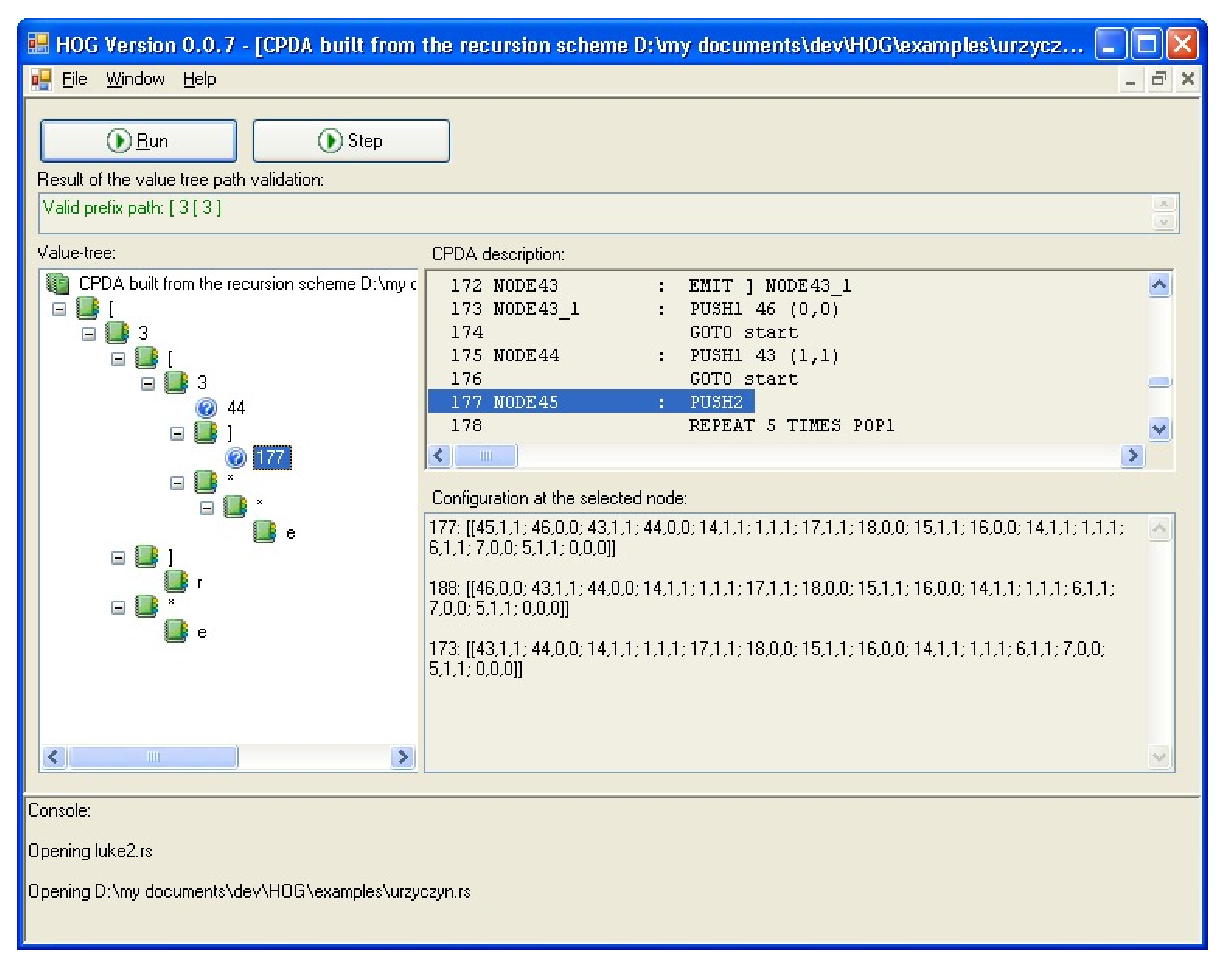
\includegraphics[width=14cm]{sshot_cpda}\\
\end{bigcenter}
  \caption{\toolname\ executing the CPDA generated from the Urzyczin recursion scheme.}
  \label{fig:sshot_cpda}
\end{figure}

Initially, the root node is labeled with the instruction number $0$ which corresponds to the first instruction of the CPDA code. When executing the CPDA transition on a node, the stack is updated accordingly and the node label is updated to the next instruction to be executed. This process is repeated until reaching an {\tt EMIT} instruction.

When an instruction $\mathtt{EMIT\ f\ LAB_1 \ldots LAB_k}$ is executed (which means that a terminal $f:o^k\rightarrow o$ is emitted), a node labelled $f$ is created in the value tree with $k$ children nodes are attached to it. Each child corresponds to a newly spawn CPDA with the same stack as in the original configuration. Finally, the current instruction of the  $i$th child is set to the instruction number with label $\mathtt{LAB_i}$.

Terminal nodes represent the actual nodes of the value-tree and as such cannot be expanded further.

\subsubsection{Exploring the tree generated by a recursion scheme}

\toolname\ has another feature which allows one to explore the infinite tree generated from a given recursion scheme without the need to convert it into a CPDA beforehand.


    \bibliographystyle{plain}
    \bibliography{../bib/dphil-all}

\end{document}

\def\toolname{HOG}

\title{A Concrete Presentation of Game Semantics}

\author{W.~Blum\thanks{Oxford University Computing Laboratory (OUCL), Wolfson Building, Parks Road, Oxford OX1 3QD, UK. {\tt william.blum@comlab.ox.ac.uk}}~~~~~~~~~~~C.-H.~L.~Ong\thanks{OUCL. {\tt Luke.Ong@comlab.ox.ac.uk}}}
\date{}


\begin{document}
\maketitle \thispagestyle{empty}

\begin{abstract}
We briefly present a new representation theory for game semantics which is very concrete: instead of playing in an arena game in which P plays the innocent strategy given by a term, the same game is played out over (a souped up version of) the abstract syntax tree of the term itself. The plays that are thus traced out are called \emph{traversals}. More abstractly, traversals are the justified sequences that are obtained by performing parallel-composition \emph{less} the hiding. After stating and explaining a number of Path-Traversal Correspondence Theorems, we present a tool for game semantics based on the new representation.
\end{abstract}

%\tableofcontents

\section{Introduction}

In game semantics, programs are modelled as strategies (for the player P). Strategies, which are certain sets of \emph{plays} (or \emph{legal positions}), are composed by \emph{parallel composition plus hiding}, in the sense of the process algebra CSP \cite{Hoa85}. The starting point of our work is a kind of representation theory of the game semantics of higher-type programs (such as recursion schemes, PCF and Idealized Algol) that is very concrete, involving combinatorics over infinite structures defined by the abstract syntax trees of the programs being modelled. Take a program $M$ which may be open. In this approach the strategy-denotation of $M$, written $\mng{M}$, is represented by a set $\travset{M}$ of \emph{traversals} over a possibly infinite tree -- called the \emph{computation tree} of $M$ -- which is generated from (a souped up version of) the abstract syntax tree of $M$. (Formally a traversal over a tree is a sequence of nodes starting from the root; quite unlike a path in the tree, a traversal can ``jump'' all over the tree, and may visit certain nodes infinitely often.) A traversal over the computation tree of $M$ does not correspond to a play in $\mng{M}$, but rather to an \emph{interaction sequence} that is obtained by \emph{uncovering} \cite{HO00} a play in $\mng{M}$ in a hereditary fashion; and a suitable projection of the traversals given by $M$ -- corresponding to the operation of hiding -- gives the strategy-denotation $\mng{M}$. We call such a result a \emph{Path-Traversal Correspondence Theorem}. (Denoting programs by sets of interaction sequences obtained by hereditary uncovering was first considered by Greenland in his DPhil thesis \cite{Gre05}, which he has called \emph{revealed semantics}.) The set $\travset{M}$ is defined by recursion over the syntax of $M$ and by rule induction.
%E.g.~in the case of recursion schemes, there is one rule for each of the four syntactic constructs.
Intuitively these formation rules define what amounts to the composition algorithm of innocent strategies (less the hiding) but expressed in a setting in which moves (of the innocent game) are mapped to nodes of the computation tree. As a consequence of the representation, instead of the arena game in which P participates by playing the innocent strategy given by a term, the same game can be played out very concretely over (a souped up version of) the abstract syntax tree of the term itself (which we call the computation tree).

This view of game semantics and the theory of traversals were first developed to prove a theorem in the verification of infinite structures (namely, ranked trees generated by higher-order recursion schemes have decidable MSO theories, in \cite{OngLics2006}). The theory has at least two other applications. First it justifies the game characterization of the Higher-Order Matching Problem (but NOT the algorithm) developed by Colin Stirling. Secondly it underpins the (as yet unpublished) result that for each $n \geq 0$, the following are equi-expressive for generating ranked trees:
\begin{enumerate}
\item order-$n$ recursion schemes (= order-$n$ PCF terms generated from uninterpreted order-1 symbols)

\item order-$n$ collapsible pushdown automata (CPDA)

\item order-$n$ pure innocent strategies.
\end{enumerate}

In this paper, after an introduction to traversals, we describe a tool that illustrates the representation theory, briefly demonstrating its capabilities. The tool can perform the inter-translations between CPDA and recursion schemes; it demonstrates the path-traversal correspondence in the form of a 2-player game in which the user can play against a given term interactively, over the computation tree of the term. Finally the tool is an aid to the type-setting of justified sequences.

\section{Computation tree, Traversals and the Correspondence Theorem}

In \cite{OngLics2006}, one of us introduced the notion of computation tree and traversals over a computation tree for the purpose of studying trees generated by higher-order recursion scheme. Here we extend these concepts to the pure (\ie without constants) simply-typed lambda calculus. Our setting allows the presence of free variable of any order. Moreover the term studied is not necessarily of ground type. (This contrasts with \cite{OngLics2006}'s setting where the term is of ground type and contains only \emph{uninterpreted constant}\footnote{A constant $f$ is  \emph{uninterpreted} if the small-step semantics of the language
  does not contain any rule of the form $f \dots \rightarrow e$. $f$
  can be regarded as a data constructor.} of order 1 at most and no
free variables.) Note that our setting automatically accounts for the presence of uninterpreted constants since they can be regarded as free variables. We will then state the \emph{Correspondence Theorem} (Theorem \ref{thm:correspondence}).

In the following we fix a simply-typed term $\Gamma \vdash M :T$.

\subsection{Computation tree}
 In \cite{OngLics2006} the computation tree of a grammar is
defined as the unravelling of a finite graph representing the long transform of a grammar. Similarly we define the computation tree of a $\lambda$-term as an abstract syntax tree of its $\eta$-long normal form.  We write $l\langle t_1, \ldots, t_n \rangle$ with $n \geq 0$ to denote the tree with a root labelled $l$ with $n$ children subtrees $t_1$, \ldots, $t_n$.

\begin{definition}\rm
\label{dfn:comptree}
  The \defname{computation tree} $\tau(M)$ of a simply-typed term
  $\Gamma \vdash M:T$ with variable names in a countable set
  $\mathcal{V}$ is a tree with labels in $ \{ @ \} \union \mathcal{V}
  \union \{ \lambda x_1 \ldots x_n \ | \ x_1 ,\ldots, x_n \in
  \mathcal{V}, n\in\nat \}$ defined from its $\eta$-long form as follows.
  Let $\overline{x}$ denote some list of variables $x_1 \ldots x_n$ for some $n\geq 0$.
\begin{eqnarray*}
  \mbox{For $m\geq 0$, $z \in \mathcal{V}$: } \tau(\lambda \overline{x} . z s_1 \ldots s_m ) &=& \lambda \overline{x} \langle z \langle\tau(s_1),\ldots,\tau(s_m)\rangle\rangle \\
  \mbox{For $m \geq 1$: } \tau(\lambda \overline{x} . (\lambda y.t) s_1 \ldots s_m) &=& \lambda \overline{x} \langle @ \langle \tau(\lambda y.t),\tau(s_1),\ldots,\tau(s_m) \rangle \rangle \ .
\end{eqnarray*}
\end{definition}

Even-level nodes are $\lambda$-nodes (the root is on level 0). A single $\lambda$-node can represent several consecutive variable abstractions or it can just be a \emph{dummy lambda} if the corresponding subterm is of ground type.  Odd-level nodes are variable or application nodes.

We say that a variable node $n$ labelled $x$ is \defname{bound} by a node $m$, and $m$ is called the \defname{binder} of $n$, if $m$ is the closest node in the path from $n$ to the root such that $m$ is labelled $\lambda \overline{\xi}$ with $x\in \overline{\xi}$.


We write $\theroot$ to denote the root of the computation tree $\tau(M)$. The set of nodes of the computation tree is denoted by $N$. The sets $N_@$, $N_\lambda$ and $N_{\sf var}$ are the subset of $N$ consisting of the @-nodes, $\lambda$-nodes and variable nodes respectively.


\subsection{Justified sequences of nodes}

We define the \defname{enabling relation} on the set of nodes of the computation tree as follows: $m$ enables $n$, written $m \vdash n$, if and only if $n$ is bound by $m$ (and we sometimes write $m \vdash_i n$ to precise that $n$ is the $i^{\sf th}$ variable bound by $m$); or $m$ is the root $\theroot$ and $n$ is a free variable; or $n$ is a $\lambda$-node and $m$ is its parent node.


We say that a node $n_0$ of the computation tree is
\defname{hereditarily enabled} by $n_p \in N$ if there are nodes
$n_1,\ldots, n_{p-1} \in N$ such that $n_{i+1}$ enables $n_{i}$ for all $i\in 0..p-1$.

For any set of nodes $S, H \subseteq N$ we write $S^{H\vdash}$ for $S \inter \vdash^*(H) = \{ n \in S \ | \exists n_0 \in H \mbox{ s.t. }n_0  \vdash^* n \}$ -- the subset of $S$ constituted of nodes hereditarily enabled by some node in $H$. We will abbreviate $S^{\{n_0\}\vdash}$ into $S^{n_0\vdash}$.

We call \defname{input-variables nodes} the elements of $V_{\sf var}^{\theroot\vdash}$ \ie variables that are hereditarily enabled by the root of $\tau(M)$. Thus we have $V_{\sf var}^{\theroot\vdash} = V \setminus ( V_{\sf var}^{N_@\vdash} \union V_{\sf var}^{N_\Sigma\vdash})$.

A \defname{justified sequence of nodes} is a sequence of nodes with pointers such that each occurrence of a variable or $\lambda$-node $n$ different from the root has a pointer to some preceding occurrence $m$ verifying $m \vdash n$. In particular, occurrences of @-nodes do not have pointer. We represent the pointer in the sequence as follows \Pstr[0.4cm]{ (m){m} \ldots (n-m,45:i) n }.
 where the label indicates that either $n$ is labelled with the $i$th variable
abstracted by the $\lambda$-node $m$ or that $n$ is the $i^{\sf th}$ child of $m$.  Children nodes are numbered from $1$ onward except for @-nodes where it starts from $0$. Abstracted variables are numbered from $1$ onward. The $i^{\sf th}$ child of $n$ is denoted by $n.i$.

We say that a node $n_0$ of a justified sequence is
\defname{hereditarily justified} by $n_p$ if there are occurrences $n_1,
\ldots, n_{p-1}$ in the sequence such that $n_i$ points to $n_{i+1}$ for all $i\in 0..p-1$. Let $n$ be an occurrence in a justified sequence $s$. We write $s \filter r$ to denote the subsequence of $s$ consisting of the occurrences hereditarily justified by $n$.


The notion of \defname{P-view} $\pview{t}$ of a justified sequence of nodes $t$ is defined the same way as the P-view of a justified sequences of moves in Game Semantics:\footnote{ The equalities in the
  definition determine pointers implicitly. For instance in the second
  clause, if in the left-hand side, $n$ points to some node in $s$
  that is also present in $\pview{s}$ then in the right-hand side, $n$
  points to that occurrence of the node in $\pview{s}$.}
$$\begin{array}{rclrcl}
\pview{\epsilon} &=&  \epsilon & \pview{\Pstr[0.5cm]{ s \cdot (m) m \cdot \ldots \cdot (lmd-m,40){\lambda\overline{\xi}} }}
 &=& \Pstr{
\pview{s} \cdot (m2) m \cdot (lm2-m2,50) {\lambda \overline{\xi}} } \\
\mbox{for $n \notin N_\lambda$, } \pview{s \cdot n }  &=&  \pview{s} \cdot n \qquad & \pview{s \cdot \theroot }  &=&  \theroot
\end{array}$$

The O-view of $s$, written $\oview{s}$, is defined dually. We will borrow the game semantic terminology: A justified sequences of nodes satisfies \defname{alternation} if for any two consecutive nodes one is a $\lambda$-node and the other is not, and \defname{P-visibility} if every variable node points to a node occurring in the P-view a that point.

\subsection{Adding value-leaves to the computation tree}

We now add another ingredient to the computation tree that was not originally used in \cite{OngLics2006}.  We write $\mathcal{D}$ to denote the set of values of the base type $o$.  We add
\defname{value-leaves} to $\tau(M)$ as follows: For each value $v
\in \mathcal{D}$ and for each node $n \in N$ we attach the child leaf $v_n$ to $n$.  We write $V$ for the set of vertices of the resulting tree (\ie inner nodes and leaf nodes). For $\$$ ranging in $\{@, \lambda, var \}$, we write $V_\$$ to denote the set of inner nodes from $N_\$$ plus the leaf-nodes whose parent is in $N_\$$ \ie $V_\$ = N_\$ \union \{ v_n \ | \ n \in N_\$, v \in \mathcal{D} \}$.


Everything that we have defined can be lifted to this new version of computation tree. The enabling relation $\vdash$ is extended so that every leaf is enabled by its parent node. A link going from a value-leaf $v_n$ to a node $n$ is labelled by $v$: \Pstr[0.4cm]{ (n) n \ldots (vn-n,35:v){v_n} }. For the definition of P-view and visibility, value-leaves are treated as $\lambda$-nodes if they are at an odd level in the computation tree, and as variable nodes if they are at an even level.

We say that an occurrence of an inner node $n \in N$ is
\defname{answered} by an occurrence $v_n$ if $v_n$ in
the sequence that points to $n$, otherwise we say that $n$ is
\defname{unanswered}. The last unanswered node is called the
\defname{pending node}.  A justified sequence of nodes is
\defname{well-bracketed} if each value-leaf occurring in it is justified by the pending node at that point.  If $t$ is a traversal then we write
$?(t)$ to denote the subsequence of $t$ consisting only of unanswered nodes.

\subsection{Traversals of the computation tree}
\label{subsec:traversal}

A \emph{traversal} is a justified sequence of nodes of the computation tree where each node indicates a step that is taken during the evaluation of the term.

\begin{definition}[Traversals for simply-typed $\lambda$-terms] \rm
\label{def:traversal} The set $\travset(M)$ of \defname{traversals}
over $\tau(M)$ is defined by induction over the rules of Table
\ref{tab:trav_rules}. A traversal that cannot be extended by any
rule is said to be \emph{maximal}.
\end{definition}

\begin{FramedTable}
\noindent {\bf Initialization rules}
\begin{itemize}[]
\item\rulenamet{Empty} $\epsilon \in \travset(M)$.
\item\rulenamet{Root} The sequence constituted of a single occurrence of $\tau(M)$'s root is a traversal.
\end{itemize}

\noindent {\bf Structural rules}
\begin{itemize}[]
    \item \rulenamet{Lam} If $t \cdot \lambda \overline{\xi}$ is a traversal then so is
        $t \cdot \lambda \overline{\xi} \cdot n$ where $n$
        denotes $\lambda \overline{\xi}$'s child and:
        \begin{compactitem}
            \item If $n \in N_@ \union N_\Sigma$ then it has no justifier;
            \item if  $n \in N_{\sf var}\setminus N_{\sf fv}$ then it points to the only occurrence\footnote{Prop.\ \ref{prop:pviewtrav_is_path} will show that P-views
            are paths in the tree thus $n$'s enabler occurs
            exactly once in the P-view.} of its binder in
            $\pview{t\cdot \lambda \overline{\xi}}$;
            \item if  $n \in N_{\sf fv}$ then it points
            to the only occurrence of the root $\theroot$ in
            $\pview{t \cdot \lambda \overline{\xi}}$.
        \end{compactitem}
    \item \rulenamet{App} If $t \cdot @$ is a traversal then so is \Pstr[0.4cm]{t \cdot (m) @  \cdot (n-m,40:0) n}.
\end{itemize}

\emph{\bf Input-variable rules}
\begin{itemize}[]
\item \rulenamet{InputVar} If $t$ is a traversal where $t^\omega \in N_{\sf var}^{\theroot\vdash} \union L_\lambda^{\theroot\vdash}$
and $x$ is an occurrence of a variable node in $\oview{t}$ then
so is $t \cdot n$ for any child $\lambda$-node $n$ of $x$, $n$
pointing to $x$.



\item \rulenamet{InputValue} If $t_1
\cdot x \cdot t_2$ is a traversal with pending node $x \in
N_{\sf var}^{\theroot\vdash}$ then so is \Pstr[0.5cm]{t_1 \cdot
(x){x} \cdot t_2 \cdot (xv-x,38:v){v_x} } for all $v \in
\mathcal{D}$.
\end{itemize}

\emph{\bf Copy-cat rules}
\begin{itemize}[]
\item\rulenamet{Var}
If \Pstr[0.5cm]{t \cdot (n){n} \cdot (lx){\lambda \overline{x}}
    \ldots (x-lx,50:i){x_i} } is a traversal where $x_i \in
    N_{\sf var}^{@\vdash}$ then so is \Pstr[0.5cm]{ t \cdot
(n){n} \cdot (lx){\lambda \overline{x}}  \ldots (x-lx,30:i){x_i}
    \cdot (letai-n,40:i){\lambda \overline{\eta_i}}
     }.

\item\rulenamet{Value}
  If \Pstr{t \cdot (m){m} \cdot (n){n}  \ldots
(vn-n,60:v){v}_{n} } is a traversal where $n\in N$ then so is
\Pstr[0.6cm]{t \cdot (m){m} \cdot (n){n} \ldots
(vn-n,60:v){v}_{n} \cdot (vm-m,45:v){v}_m}.
\end{itemize}
\caption[Traversal rules for the simply-typed
lambda-calculus]{Traversal rules for the simply-typed
$\lambda$-calculus.}
 \label{tab:trav_rules}
\end{FramedTable}


\parpic[r]{
 $\pssetcomptree\tree[levelsep=3ex,treesep=0.5cm]{\lambda} {
    \tree{@}{
        \pstree[linestyle=dotted]{\TR{\lambda y}\arclabel{0} }{
            \tree{y}{
                \tree{\lambda \overline{\eta_1}}{\vdots}%\arclabel{1}
                \tree{\lambda \overline{\eta_i}}{\vdots}%\arclabel{i}
                \tree{\lambda \overline{\eta_n}}{\vdots}%\arclabel{n}
            }
        }
        \pstree[linestyle=dotted]{\TR{\lambda \overline{x}}
            \arclabel{1}}{ \tree{x_i}{\TR{} \TR{}}}
}}$ } A traversal always starts by visiting the root. Then it mainly follows the structure of the tree. The (Var) rule permits to jump across the computation tree. The idea is that after visiting a variable node $x$, a jump is allowed to the node corresponding to the subterm that would be substituted for $x$ if all the $\beta$-redexes occurring in the term were reduced. The sequence \Pstr[0.8cm]{\lambda \cdot (app) @  \cdot (ly) {\lambda y}  \ldots (y-ly,35:1) y  \cdot (lx-app,38:1) {\lambda \overline{x}} \ldots (x-lx,30:i) {x_i} \cdot (leta-y,40:i) {\lambda \overline{\eta_i} } \ldots}
 is an example of traversal of the computation tree shown on the right.

\begin{proposition}[counterpart of proposition 6 from \cite{OngHoMchecking2006}]
\label{prop:pviewtrav_is_path} Let $t$ be a traversal. Then:
\begin{enumerate}[(i)]
\item $t$ is a well-defined and well-bracketed justified sequence;
\item $t$ is a well-defined justified sequence verifying alternation, P-visibility and O-visibility;
\item If $t$'s last node is not a value-leaf, then $\pview{t}$ is the path in the computation tree going from the root to $t$'s last node.
\end{enumerate}
\end{proposition}

The \defname{reduction} of a traversal $t$ is the subsequence of $t$ obtained by keeping only occurrences of nodes that are hereditarily enabled by the root $\theroot$. This has the effect of eliminating the ``internal nodes'' of the computation. If $t$ is a non-empty traversal then the root $\theroot$ occurs exactly once in $t$ and the reduction of $t$ is equal to $t \filter r$. We write $\travset(M)^{\filter \theroot}$ for the set or reduction of traversals of $M$.

Application nodes are used to connect the operator and the operand of an application in the computation tree but since they do not play any role in the computation of the term, we can remove them from the traversals.  We write $t-@$ for the sequence of nodes-with-pointers obtained by removing from $t$ all @-nodes and value-leaves of @-nodes, any link pointing to an @-node being replaced by a link pointing to the immediate predecessor of @ in $t$. We write $\travset(M)^{-@}$ for the set $\{ t - @ \ | \  t \in \travset(M) \}$.
\begin{remark}
If $M$ is $\beta$-normal then $\tau$ does not contain any @-node therefore all nodes are hereditarily justified by $r$ and we have $\travset(M)^{-@} = \travset(M) = \travset(M)^{\filter \theroot }$.
\end{remark}

\subsection{Revealed Game Semantics}

In game semantics, strategy composition is achieved by performing a CSP-like ``composition + hiding''. If the internal moves are not hidden then we obtain an alternative semantics called \emph{revealed semantics} in \cite{willgreenlandthesis} and \emph{interaction} semantics in \cite{DBLP:conf/sas/DimovskiGL05}. Here we will refer to this semantics as the \defname{fully revealed game semantics}. The fully revealed game denotation of a term $\Gamma \vdash M :T$, written $\revsem{\Gamma \vdash M : T}$, is obtained by uncovering\footnote{An algorithm that uniquely recovers hidden moves is given in Part II of
  \cite{hylandong_pcf}.} all the internal moves from $\sem{\Gamma \vdash
  M : T}$ generated during strategy composition.
We introduce a variation of the fully-revealed game denotation called the \defname{syntactically-revealed game denotation}, written $\syntrevsem{\Gamma \vdash
  M : T}$. In this denotation, as opposed to the fully-revealed denotation,
only \emph{certain} internal moves from $\sem{\Gamma \vdash
  M : T}$ are uncovered: The internal moves that are generated by the composition with the evaluation map
$ev$ at a @-node of the computation tree are all uncovered, but in the denotation of a subtem of the form $y N_1 \ldots N_p$ for some $p\geq1$, only certain internal moves are uncovered. The formal definition can be found in \cite{localbeta2008}.

\subsection{Computation trees and arenas}
We consider the well-bracketed game model of the simply-typed lambda calculus.  We choose to represent strategies using ``prefix-closed set of plays''. \footnote{In the literature, a strategy is usually defined as a set of plays closed by \emph{even}-length prefix. For the purpose of showing the Correspondence Theorem, however, the ``prefix-closed''-based definition is more adequate.} We fix a term $\Gamma \vdash M : T$ and write $\sem{\Gamma \vdash M : T}$ for its strategy denotation. The answer moves of a question $q$ are written $v_q$ where $v$ ranges in $\mathcal{D}$.

\begin{proposition}
There exists a function $\varphi_M$, constructible from $\tau(M)$, that maps nodes from $V\setminus (V_@ \union V_\Sigma)$ to moves of the interaction arena underlying the revealed strategy $\syntrevsem{\Gamma \vdash M : T}$ and such that $\varphi$ maps $\lambda$-nodes to O-questions, variable nodes to P-questions, value-leaves of $\lambda$-nodes to P-answers and value-leaves of variable nodes to O-answers.
\end{proposition}

\begin{example}
Take $\lambda x . (\lambda g . g x) (\lambda y . y)$ with $x,y:o$ and $g:(o,o)$. The diagram below represents the computation tree (middle), the arenas $\sem{(o,o), o}$ (left), $\sem{o , o}$ (right), $\sem{o\rightarrow o}$ (rightmost) and $\varphi = \psi \union \psi_{\lambda g.g x}^{\lambda g, q_{\lambda g}} \union \psi_{\lambda y.y}^{\lambda y, q_{\lambda y}}$ (dashed-lines).
$$\psset{levelsep=3.5ex}
\pstree{\TR[name=root]{\lambda x}} {
    \pstree{\TR[name=App]{@}}
    {
            \pstree{\TR[name=lg]{\lambda g}}
                { \pstree{\TR[name=lgg]{g}}{
                        \pstree{\TR[name=lgg1]{\lambda}}
                        { \TR[name=lgg1x]{x}  } } }
            \pstree{\TR[name=ly]{\lambda y}}
                    {\TR[name=lyy]{y}}
    }
} \rput(4.5cm,-1cm){
  \pstree{\TR[name=A1lx]{q_{\lambda x}}}
        { \TR[name=A1x]{q_x} }
} \rput(-6cm,-1.5cm){
    \pstree{\TR[name=A2lg]{q_{\lambda g}}}
    {
        \pstree{\TR[name=A2g]{q_g}}
        {  \TR[name=A2g1]{q_{g_1}}   }
    }}
\rput(2.5cm,-1.5cm){
    \pstree{\TR[name=A3ly]{q_{\lambda y}}}
        { \TR[name=A3y]{q_y}
        }
} \psset{nodesep=1pt,arrows=->,arcangle=-20,arrowsize=2pt 1,linestyle=dashed,linewidth=0.3pt} \ncline{->}{root}{A1lx} \mput*{\psi} \ncarc{->}{lgg1x}{A1x} \ncline{->}{lg}{A2lg} \mput*{\psi_{\lambda g.g x}^{\lambda g, q_{\lambda g}}} \ncline{->}{lgg}{A2g} \ncline{->}{lgg1}{A2g1} \ncline{->}{ly}{A3ly} \mput*{\psi_{\lambda y.y}^{\lambda y, q_{\lambda y}}} \ncline{->}{lyy}{A3y}
$$
\end{example}

We extend the function $\varphi$ to justified sequences of nodes as follows: If $t = t_0 t_1 \ldots$ is a justified sequence of nodes in $V_\lambda \union V_{\sf var}$ then $\varphi(t)$ is defined to be the sequence of moves $\varphi(t_0)\ \varphi(t_1) \ldots$ equipped with the pointers of $t$.


\subsection{The Correspondence Theorem}


In the simply-typed lambda calculus, the set $\travset(M)$ of traversals of the computation tree is isomorphic to the set of plays of the syntactically-revealed denotation. Moreover the set of traversal reductions is isomorphic to the standard strategy denotation:

\begin{theorem}[The Correspondence Theorem]
\label{thm:correspondence} The function $\varphi_M$ gives us the following two isomorphisms:
\begin{eqnarray*}
(i)~\varphi_M  &: \travset(M)^{-@} \stackrel{\cong}{\longrightarrow} \syntrevsem{\Gamma \vdash M :T} \\
(ii)~\varphi_M  &: \travset(M )^{\filter \theroot} \stackrel{\cong}{\longrightarrow} \sem{\Gamma \vdash M : T} \ .
\end{eqnarray*}
\end{theorem}

\begin{example}
Take $M = \lambda f z . (\lambda g x . f x) (\lambda y. y) (f z) : ((o,o),o, o)$.  The figure below represents the computation tree (left tree), the arena $\sem{((o,o),o, o)}$ (right tree) and $\psi_M$ (dashed line). (Only question moves are shown for clarity.) The justified sequence of nodes $t$ defined hereunder is an example of traversal:

\begin{tabular*}{\textwidth}{lcp{6.3cm}}
$\pssetcomptree\pstree[levelsep=2.5ex,treesep=0.3cm]{ \TR[name=root]{\lambda f z} }
     {  \tree[levelsep=4ex]{@}
        {   \tree{\lambda g x}{
                  \pstree{\TR[name=f]{f^{[1]}}}{
                            \pstree{\TR[name=lmd]{\lambda^{[2]}}}
                                {\TR{x}}
                  }
                }
            \tree{\lambda y }{\TR{y}}
            \tree{\lambda ^{[3]}}{
                \pstree{\TR[name=f2]{f^{[4]}}} {
                \pstree{\TR[name=lmd2]{\lambda^{[5]}}}{\TR[name=z]{z}}
                }
            }
        }
     }
\hspace{1cm}
  \pstree[levelsep=8ex, treesep=0.3cm]{ \TR[name=q0]{q^0} }
    {   \pstree[levelsep=4ex]{\TR[name=q1]{q^1}} {\TR[name=q2]{q^2}}
        \TR[name=q3]{q^3}
    }
\psset{nodesep=1pt,arrows=->,arrowsize=2pt 1,linestyle=dashed,linewidth=0.3pt} \ncline{->}{root}{q0} \mput*{\psi_M} \ncarc[arcangle=-25]{->}{z}{q3} \ncarc[arcangle=10]{->}{f}{q1} \ncarc[arcangle=10]{->}{lmd}{q2} \ncline{->}{f2}{q1} \ncline{->}{lmd2}{q2}$ &  &
\begin{asparablank}
  \item  \Pstr[0.8cm]{
t = (n){\lambda f z} \ (n2){@} \ (n3-n2,60){\lambda g x} \ (n4-n,45){f^{[1]}} \ (n5-n4,45){\lambda^{[2]}} \ (n6-n3,45){x} \ (n7-n2,35){\lambda^{[3]}} \ (n8-n,35){f^{[4]}} \ (n9-n8,45){\lambda^{[5]}} \ (n10-n,35){z} }

\item \Pstr[0.9cm]{
t\filter r = (n){\lambda f z} \ (n4-n,50){f}^{[1]} \ (n5-n4,60){\lambda}^{[2]} \ (n8-n,45){f}^{[4]} \ (n9-n8,60){\lambda}^{[5]} \ (n10-n,40){z}}
\item
\Pstr[0.8cm]{ {\varphi_M(t\filter r) =\ } (n){q^0}\ (n4-n,60){q^1}\ (n5-n4,60){q^2}\ (n8-n,45){q^1}\ (n9-n8,60){q^2}\ (n10-n,38){q^3} \in \sem{M}\ .}
\end{asparablank}
\end{tabular*}
\end{example}


\section{Presentation of the tool}

We have developed a tool called \toolname\ that permits one to visualize and explore the Traversal-Game Semantics Correspondence presented in the previous section. The binary files and sources in OCaml/F\# can be downloaded from \url{http://web.comlab.ox. ac.uk/oucl/work/william.blum/}.

\subsection{Generation of the computation graph/tree}

\toolname\ accepts two kind of objects as an input: simply-typed terms or higher-order recursion schemes. A recursion scheme is a special kind of higher-order grammar that can be used to generated an infinite tree called the value-tree (not to be confused with the computation tree). A recursion scheme can be thought as a simply-typed term of ground type extended with recursion and containing uninterpreted constant of order at most 1 (used to represent the constructors for the nodes of the value tree). Since recursion schemes allow the use of recursion, the computation tree becomes a computation \emph{graph}. Traversals are however defined in the same way and the Correspondence Theorem still holds. This setting was originally treated in \cite{OngLics2006} where the concepts of computation tree and traversal were introduced.


\toolname\ allows you to generate the computation tree of a higher-order simply-typed term as well as the computation graph of a higher-order recursion scheme.

\subsection{Example}

Take for instance the Urzyczin recursion scheme (see \cite{demirandathesis}). It is formally given by the tuple $\langle \Sigma, \mathcal{N}, \mathcal{R}, S \rangle $ where the set of terminals is $\Sigma = \{[:o\typear o,
    ]:o \typear o,*:o \typear o, 3:o \typear o \typear o \typear o, e:o,
    r:o\}$, the set of non-terminals is
 $\mathcal{N} = \{ S:o,
    D:(o \typear o \typear o) \typear o \typear o \typear o \typear
    o,
    F:o \typear o,
    E:o,
    G:o \typear o \typear o \}$ and the set of rules $\mathcal{R}$ is given by
\[\begin{array}{rll}
   S\, & \rightarrow & [\, (D\, G\, E\, E\, E\,) \\
    D\, \varphi x y z & \rightarrow & 3 ([ (D\, (D\, \varphi\, x)\, z\, (F\, y) (F\, y))) (] (\varphi\, y\, x)) (* z) \\
    F\, x & \rightarrow & *\, x \\
    E\, & \rightarrow & e \\
    G\, u v & \rightarrow & r
\end{array}\]


Using the \toolname\ syntax this is expressed as follows:
\begin{lstlisting}[breaklines=true]
name { "Urzyczin tree" } validator { demiranda_urzyczyn } terminals{
    [:o-> o;
    ]:o -> o;
    *:o -> o;
    3:o -> o -> o -> o;
    e:o;
    r:o; }
nonterminals {
    S:o ;
    D:(o -> o -> o) -> o -> o -> o -> o ;
    F:o -> o ;
    E:o;
    G:o -> o -> o; }
rules {
    S = [ (D G E E E) ;
    D \varphi x y z = 3 ([ (D (D \varphi x) z (F y) (F y))) (] (\varphi y x)) (* z);
    F x = * x ;
    E = e ;
    G u v = r ; }
\end{lstlisting}

Figure \ref{fig:urz_graph} represents the computation graph. (The \TeX\ source code for this graph is automatically generated by \toolname.) The framed nodes correspond to the constant nodes.

\begin{figure}[htbp]
\begin{bigcenter}
\psset{levelsep=5ex,linewidth=0.5pt,nodesep=1pt,arcangle=-20,arrowsize=2pt 1} \setlength\fboxsep{2pt}
%\newcommand{\pssetcomptree}{\psset{levelsep=4ex,linewidth=0.5pt}}
\pssetcomptree $\pstree{\TR{[S]\lambda }}{\pstree{\TR{\framebox{[}}}{\pstree{\TR{\lambda }}{\pstree{\TR{@}}{\pstree{\TR[name=1]{[D]\lambda \varphi x y z}\ncput*{\scriptstyle 0}}{\pstree{\TR{\framebox{3}}}{\pstree{\TR{\lambda }}{\pstree{\TR{\framebox{[}}}{\pstree{\TR{\lambda }}{\pstree{\TR[name=n0]{@}}{\pstree{\TR{\lambda \theta_{3} \theta_{4}}}{\pstree{\TR[name=n1]{@}}{\pstree{\TR{\lambda \theta_{5} \theta_{6}}}{\pstree{\TR{\varphi}}{\pstree{\TR{\lambda }}{\TR{\theta_{5}}} \pstree{\TR{\lambda }}{\TR{\theta_{6}}}}} \pstree{\TR{\lambda }}{\TR{x}} \pstree{\TR{\lambda }}{\TR{\theta_{3}}} \pstree{\TR{\lambda }}{\TR{\theta_{4}}}}} \pstree{\TR{\lambda }}{\TR{z}} \pstree{\TR{\lambda }}{\pstree{\TR{@}}{\pstree{\TR[name=2]{[F]\lambda x}\ncput*{\scriptstyle 0}}{\pstree{\TR{\framebox{*}}}{\pstree{\TR{\lambda }}{\TR{x}}}}\pstree{\TR{\lambda }}{\TR{y}}}} \pstree{\TR{\lambda }}{\pstree{\TR[name=n2]{@}}{\pstree{\TR{\lambda }}{\TR{y}}}}}}}} \pstree{\TR{\lambda }}{\pstree{\TR{\framebox{]}}}{\pstree{\TR{\lambda }}{\pstree{\TR{\varphi}}{\pstree{\TR{\lambda }}{\TR{y}} \pstree{\TR{\lambda }}{\TR{x}}}}}} \pstree{\TR{\lambda }}{\pstree{\TR{\framebox{*}}}{\pstree{\TR{\lambda }}{\TR{z}}}}}}\pstree{\TR{\lambda \theta_{1} \theta_{2}}}{\pstree{\TR{@}}{\pstree{\TR{[G]\lambda u v}\ncput*{\scriptstyle 0}}{\TR{\framebox{r}}}\pstree{\TR{\lambda }}{\TR{\theta_{1}}} \pstree{\TR{\lambda }}{\TR{\theta_{2}}}}} \pstree{\TR[name=3]{[E]\lambda }}{\TR{\framebox{e}}} \pstree{\TR[name=3]{[E]\lambda }}{\TR{\framebox{e}}} \pstree{\TR[name=3]{[E]\lambda }}{\TR{\framebox{e}}}}}}} \ncarc{->}{n2}{2}\ncput*{\scriptstyle 0} \ncarc{->}{n1}{1}\ncput*{\scriptstyle 0} \ncarc{->}{n0}{1}\ncput*{\scriptstyle 0}$
\end{bigcenter}
  \caption{Computation graph of the Urzyczin's recursion scheme.}
  \label{fig:urz_graph}
\end{figure}


\subsection{Playing the traversal game}

Once a computation tree/graph is loaded, \toolname\ allows you to play a traversal game over it. The user plays for the Opponent while \toolname\ plays for the Proponent. Figure \ref{fig:sshot_hog_traversal} shows a screenshot of the tool when a traversal game is played.
\begin{figure}
\begin{bigcenter}
  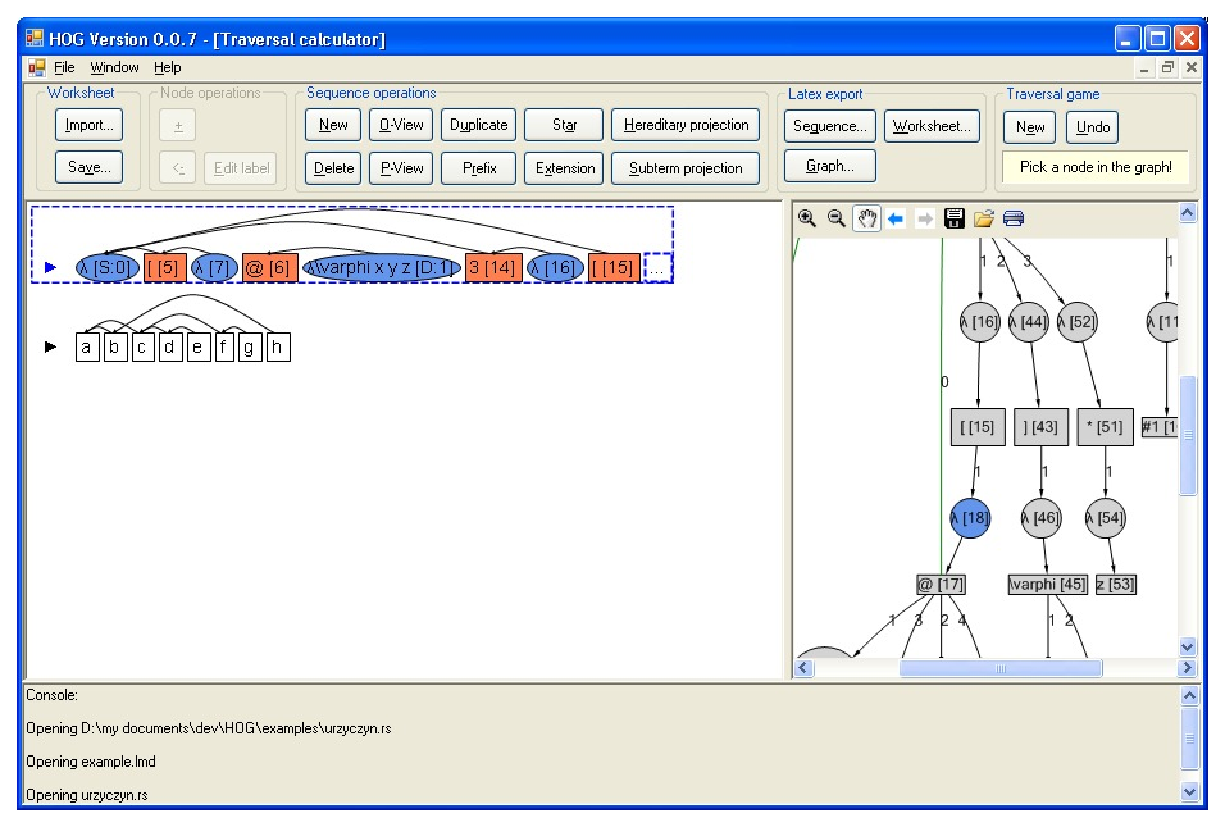
\includegraphics[width=15cm]{sshot_traversal}\\
\end{bigcenter}
  \caption{Screenshot of a traversal game in \toolname.}
  \label{fig:sshot_hog_traversal}
\end{figure}

The right-hand side of the window contains a representation of the computation graph and the left part of the window contains a list of justified sequences created by the user. In the screenshot, the first justified sequence corresponds to a traversal that is being played by the user. Opponent moves and Proponent moves are represented by circles and rectangular nodes respectively. The user make a move by selecting a node among the valid nodes highlighted in the computation graph. If there is a unique possible
 justifier in the traversal then the move is automatically
accepted, otherwise the user has to specify a move by selecting a valid justifier in the traversal. After the move is accepted \toolname\ responds with a P-move. This goes on until the traversal is maximal.

\toolname\ allows the user to perform several operations on the justified sequence such as computing the P-view or the O-view. It is also possible to export the sequence to \LaTeX\ code. For example, typesetting the traversal from Figure \ref{fig:sshot_hog_traversal} with \LaTeX\ produces
$$\Pstr[0.7cm]{(n0){\lambda }\ (n1-n0){[}\ (n2-n1){\lambda }\ (n3){@}\ (n4-n3){\lambda \varphi x y z}\ (n5-n0){3}\ (n6-n5){\lambda }\ (n7-n0){[}\ {...}\ }$$

\subsection{Other features}




\subsubsection{Generating a CPDA from a recursion scheme}
\toolname\ can  convert any higher-order recursion scheme into an equivalent (\ie generating the same infinite tree) Collapsible Push-down Automaton (CPDA) of the same order. The algorithm used to perform this transformation is taken from \cite{hague-sto07}.

The transition function of a CPDA is given by a list of instructions which we call the ``code'' of the CPDA. Figure \ref{fig:cpda_listing} give an example of CPDA generated from the Urzyczin recursion scheme.

\begin{figure}
\begin{lstlisting}[breaklines=true,basicstyle=\tiny]
Order: 2

Stack alphabet: 0 1 2 3 4 5 6 7 8 9 10 11 12 13 14 15 16 17 18 19 20 21 22 23 24 25 26 27 28 29 30 31 32 33 34 35 36 37 38 39 40 41 42 43 44 45 46 47 48 49 50 51 52 53 54 55 56 57 58 59

Code:
Code:

    0                   PUSH1 0 (0,0)
    1 start          :  CASETOP0 0->NODE0 1->NODE1 2->NODE2 3->NODE3 4->NODE4 5->NODE5 6->NODE6 7->NODE7 8->NODE8 9->NODE9 10->NODE10 11->NODE11 12->NODE12 13->NODE13 14->NODE14 15->NODE15 16->NODE16 17->NODE17 18->NODE18 19->NODE19 20->NODE20 21->NODE21 22->NODE22 23->NODE23 24->NODE24 25->NODE25 26->NODE26 27->NODE27 28->NODE28 29->NODE29 30->NODE30 31->NODE31 32->NODE32 33->NODE33 34->NODE34 35->NODE35 36->NODE36 37->NODE37 38->NODE38 39->NODE39 40->NODE40 41->NODE41 42->NODE42 43->NODE43 44->NODE44 45->NODE45 46->NODE46 47->NODE47 48->NODE48 49->NODE49 50->NODE50 51->NODE51 52->NODE52 53->NODE53 54->NODE54 55->NODE55 56->NODE56 57->NODE57 58->NODE58 59->NODE59
    2 NODE0          :  PUSH1 5 (1,1)
    3                   GOTO start
    4 NODE1          :  PUSH1 14 (1,1)
    5                   GOTO start
    6 NODE2          :  PUSH1 55 (1,1)
    7                   GOTO start
    8 NODE3          :  PUSH1 58 (1,1)
    9                   GOTO start
   10 NODE4          :  PUSH1 59 (1,1)
   11                   GOTO start
   12 NODE5          :  EMIT [ NODE5_1
   13 NODE5_1        :  PUSH1 7 (0,0)
   14                   GOTO start
   15 NODE6          :  PUSH1 1 (1,1)
   16                   GOTO start
   17 NODE7          :  PUSH1 6 (1,1)
   18                   GOTO start
   19 NODE8          :  PUSH1 4 (1,1)
   20                   GOTO start
   21 NODE9          :  PUSH1 8 (1,1)
   22                   GOTO start
   23 NODE10         :  REPEAT 3 TIMES POP1
   24                   COLLAPSE
   25                   CASETOP0 45->NODE10_45 21->NODE10_21
   26                   FAILWITH "Unexpected top 0-element!"
   27 NODE10_21      :  PUSH1 24 (3,1)
   28                   GOTO start
  ...
\end{lstlisting}
\label{fig:cpda_listing}
\caption{Excerpt of the listing of the CPDA generated  from the Urzyczin recursion scheme.}
\end{figure}

A line of code of the CPDA is made of three parts: the line number, an optional label and an instruction. There are four kinds of instructions: stack instructions, the node emitting instruction, branching instructions and debugging instructions. The stack instructions are:
\begin{description}
  \item[{\tt PUSH1 a (j,k)}] push the element {\tt a} on the top 1-stack an associates the link $(j,k)$ to it. This encoding means that the link points to a prefix stack obtained by performing an order-$j$ pop $k$ consecutive times.
  \item[{\tt PUSHn}] performs an order $n$ push on the stack (duplicates the top $n-1$-stack).
  \item[{\tt POPn}] performs an order $n$ pop on the stack (pop the top $n-1$-stack).
  \item[{\tt COLLAPSE}] collapses the stack to the prefix stack pointed to by the top element in the stack. In other words it executes $k$ times the execution {\tt POPj} where {\tt (j,k)} is the encoding of the link associated to the top element.

  \item[{\tt REPEAT n TIMES ins}] repeats the instruction {\tt ins} $n$ times where $n$ is a constant. The behaviour is unspecified if {\tt ins} is a branching instruction.
\end{description}

In order to create nodes in the value-tree, the CPDA uses teh following special instruction:
\begin{description}
  \item[$\mathtt{EMIT\ f\ LAB_1 \ldots LAB_k}$] emits the terminal $f$ of type $o^k \rightarrow o$.
   The CPDA is then spawn into $k$ other CPDA's, one for each parameter of the terminal $f$.
   The $i's$ spawn CPDA will be started at instruction $\mathtt{LAB_i}$ for $i \in \{1..k\}$.
\end{description}

The branching instructions are:
\begin{description}
  \item[{\tt GOTO lab}] jumps to the label {\tt lab}.
  \item[$\mathtt{CASTOP0\ e_0->lab_0 ... e_k->lab_k}$] performs a test case on the element
  at the top of the stack. If the top element is equal to $\mathtt{e_i}$ for some $i \in \{0..k\}$
  then the CPDA jumps to the label $\mathtt{lab_k}$. Otherwise it moves on to the following instruction.
\end{description}

There are also instructions used for debugging the code of a CPDA:
\begin{description}
  \item[{\tt FAILWITH msg}] raises an exception with the message {\tt msg}.
  \item[{\tt ASSERT msg}] asserts that the condition described by the message {\tt msg} is verified. If the test fails then an exception is raised.
\end{description}



A configuration of the CPDA is given by an instruction number together with an order-$n$ stack. In the initial configuration, the CPDA is positioned on the first instruction and the stack is the empty order-$n$ stack. After executing a transition the CPDA moves to the next instruction (or jump to another line if it is a branching instruction).




\subsubsection{Exploring the value tree by executing the CPDA transitions }

When you open a CPDA, \toolname\ displays a lazy value tree (Figure \ref{fig:sshot_cpda}). Each node of this tree corresponds to a configuration of the CPDA. Nodes are either labelled by an instruction number or by a terminal. In a separate textbox, \toolname\ shows the content of the stack for the selected configuration.

\begin{figure}
\begin{bigcenter}
  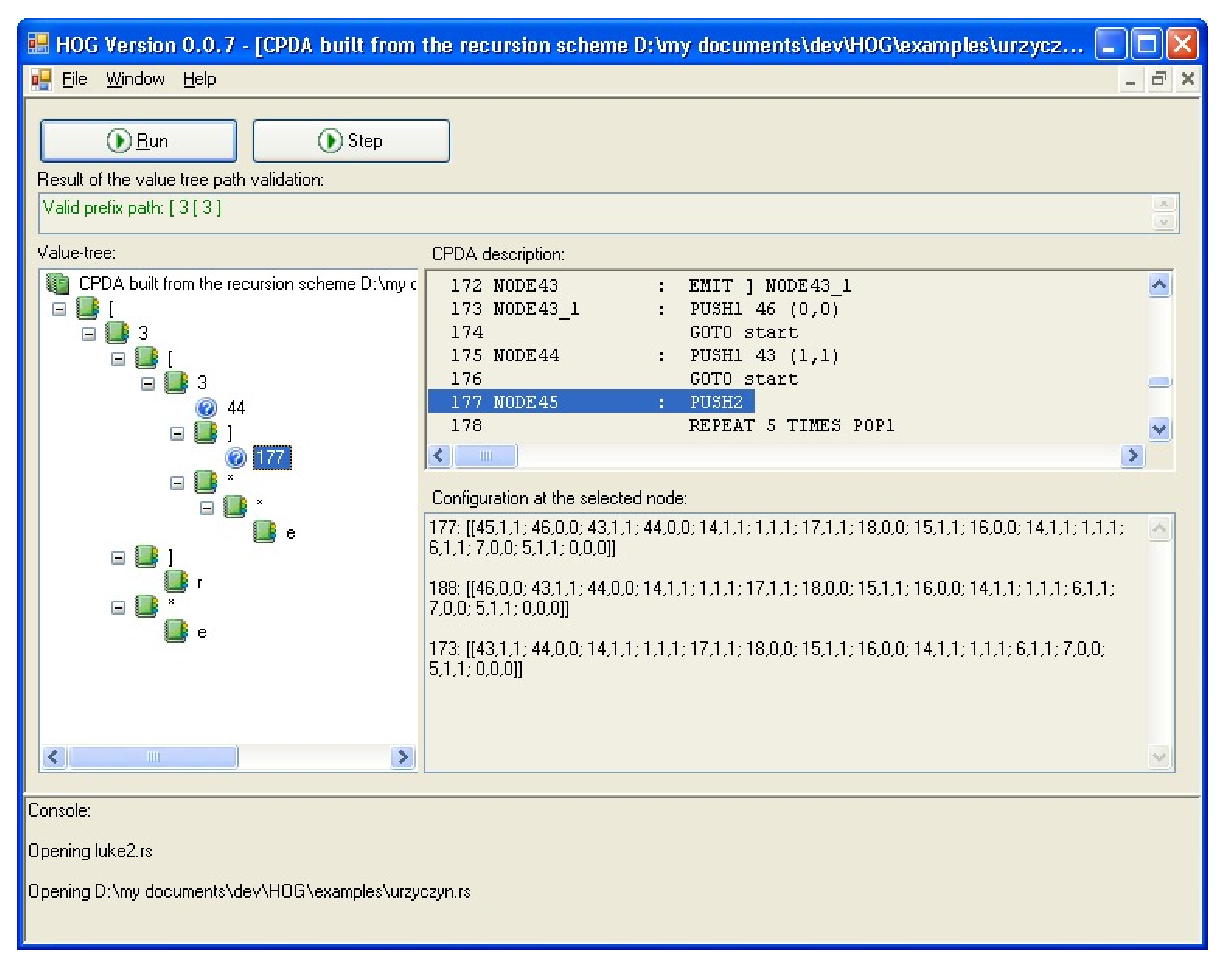
\includegraphics[width=14cm]{sshot_cpda}\\
\end{bigcenter}
  \caption{\toolname\ executing the CPDA generated from the Urzyczin recursion scheme.}
  \label{fig:sshot_cpda}
\end{figure}

Initially, the root node is labeled with the instruction number $0$ which corresponds to the first instruction of the CPDA code. When executing the CPDA transition on a node, the stack is updated accordingly and the node label is updated to the next instruction to be executed. This process is repeated until reaching an {\tt EMIT} instruction.

When an instruction $\mathtt{EMIT\ f\ LAB_1 \ldots LAB_k}$ is executed (which means that a terminal $f:o^k\rightarrow o$ is emitted), a node labelled $f$ is created in the value tree with $k$ children nodes are attached to it. Each child corresponds to a newly spawn CPDA with the same stack as in the original configuration. Finally, the current instruction of the  $i$th child is set to the instruction number with label $\mathtt{LAB_i}$.

Terminal nodes represent the actual nodes of the value-tree and as such cannot be expanded further.

\subsubsection{Exploring the tree generated by a recursion scheme}

\toolname\ has another feature which allows one to explore the infinite tree generated from a given recursion scheme without the need to convert it into a CPDA beforehand.


    \bibliographystyle{plain}
    \bibliography{../bib/dphil-all}

\end{document}
